\documentclass[11pt,a4paper]{article}
\usepackage[a4paper,margin=2.1cm]{geometry}
\usepackage[T1]{fontenc}
\usepackage{tgpagella}
\usepackage[scaled=0.92]{helvet}
\usepackage[scaled=0.86]{beramono}
\usepackage{graphicx,booktabs,longtable,array,tabularx,makecell,caption,subcaption,enumitem,amsmath,amssymb,fancyhdr,lastpage,needspace,xcolor}
\usepackage[section]{placeins}
\usepackage{fvextra}
\usepackage{tikz}
\usetikzlibrary{positioning,arrows.meta,fit,calc,shapes.geometric,backgrounds}
\usepackage[hidelinks]{hyperref}
\usepackage{titlesec}
\graphicspath{{../results/}{./}}

% ---------- monochrome house style ----------
\titleformat{\section}{\large\bfseries\sffamily}{\thesection}{0.8em}{}[\vspace{-2pt}\rule{\linewidth}{0.4pt}]
\titleformat{\subsection}{\normalsize\bfseries\sffamily}{\thesubsection}{0.8em}{}
\titleformat{\subsubsection}{\normalsize\itshape}{\thesubsubsection}{0.8em}{}
\setlength{\parindent}{0pt}
\setlength{\parskip}{5pt}
\setlength{\LTcapwidth}{\textwidth}
\setlist{nosep,leftmargin=1.4em,topsep=2pt}
\captionsetup{font=small,labelfont={bf,sf},justification=raggedright,singlelinecheck=false,skip=4pt}
\captionsetup[sub]{justification=centering,labelfont={sf}}
\renewcommand{\arraystretch}{1.15}
\renewcommand{\topfraction}{0.9}\renewcommand{\bottomfraction}{0.7}\renewcommand{\textfraction}{0.08}
\renewcommand{\floatpagefraction}{0.8}\setcounter{topnumber}{3}\setcounter{bottomnumber}{2}\setcounter{totalnumber}{5}
\newcolumntype{L}[1]{>{\raggedright\arraybackslash}p{#1}}
\newcolumntype{Y}{>{\raggedright\arraybackslash}X}
\pagestyle{fancy}\fancyhf{}
\renewcommand{\headrulewidth}{0.4pt}
\lhead{\small\sffamily OsdagBridge plate girder module -- testing report}
\rhead{\small\sffamily FOSSEE Winter Internship 2026}
\cfoot{\small\sffamily Page \thepage\ of \pageref{LastPage}}
\newcommand{\issue}[1]{\href{https://github.com/Nidhikhare12/OsdagBridge/issues/#1}{\##1}}
\newcommand{\ev}[1]{\href{https://github.com/Aditya060806/OsdagBridge/tree/screening-testing/testing/#1}{\nolinkurl{#1}}}
\newcommand{\gentab}[1]{{\footnotesize\setlength{\tabcolsep}{4pt}\input{generated/#1}}}
\newcommand{\src}[1]{\texttt{#1}}
\newcommand{\code}[1]{\VerbatimInput[frame=single,framesep=5pt,fontsize=\footnotesize,samepage=true,breaklines,breakanywhere,breaksymbolleft={},breakindent=1.5em]{#1}}

\tikzset{
  box/.style={draw,rectangle,thick,minimum height=10mm,align=center,font=\small\sffamily,fill=white,inner sep=3pt},
  gbox/.style={box,fill=gray!10},
  dbox/.style={draw,rectangle,dashed,minimum height=9mm,align=center,font=\small\sffamily,fill=gray!6,inner sep=3pt},
  store/.style={draw,cylinder,shape border rotate=90,aspect=0.22,minimum height=12mm,align=center,font=\small\sffamily,fill=gray!8,inner sep=2pt},
  arr/.style={-{Stealth[length=2.3mm]},thick},
  darr/.style={-{Stealth[length=2.3mm]},thick,dashed},
  bug/.style={draw,thick,rounded corners=1pt,fill=black,text=white,font=\scriptsize\sffamily\bfseries,inner sep=1.5pt},
  lbl/.style={font=\scriptsize\sffamily\itshape,text=black!70},
}

\begin{document}
\raggedright

% ---------------- title block ----------------
\begin{center}
{\sffamily\small FOSSEE, IIT Bombay \quad$\cdot$\quad Osdag Winter Internship 2026 \quad$\cdot$\quad OsdagBridge Software Testing \& Issue Reporting}\\[10pt]
{\LARGE\bfseries\sffamily OsdagBridge: Short-Span Steel Girder Bridge Module}\\[5pt]
{\large Functional Testing, Verification and Issue Report}\\[10pt]
Aditya Pandey \quad (GitHub \href{https://github.com/Aditya060806}{Aditya060806}) \quad 22 November 2026
\end{center}
\vspace{2pt}
\begin{tabularx}{\linewidth}{@{}lY@{}}
\toprule
Build tested & \texttt{Nidhikhare12/OsdagBridge}, branch \texttt{dev} @ \texttt{d74f56d}, source unmodified \\
Platform & Windows 11 (Intel RaptorLake GPU, OpenGL 4.6), Miniconda 26.9.4, Python 3.12.16, PySide6 6.11.3 \\
Test repository & \href{https://github.com/Aditya060806/OsdagBridge/tree/screening-testing/testing}{\nolinkurl{github.com/Aditya060806/OsdagBridge/tree/screening-testing/testing}} (collaborator: Nidhikhare12) \\
Issues filed & \issue{147}, \issue{148}, \issue{149}, \issue{150}, \issue{151}, \issue{152}; comments on \issue{20}, \issue{93}, \issue{112}, \issue{134} \\
Pull request & \issue{235}: fix and regression test for \issue{148} (open) \\
Test cases & 20 cases in 6 sessions: 15 design runs, 10 consecutive redesigns, 5 validation cases, 2 design reports, 20 \texttt{.osi} files \\
Screencast & \ev{results/demo/osdagbridge_testing_demo.mp4} (2 min 13 s, silent) \\
\bottomrule
\end{tabularx}

\section{Executive summary}
I tested the desktop GUI of the OsdagBridge plate girder module in 20 test cases over six sessions. Every design run was
driven through the real application window, with custom properties for every steel member and for the deck, and at least
three consecutive unlock--edit--redesign cycles per session. For each run I captured the UI values, the input and output
dictionaries, the material properties the analysis actually used, every Output Dock bar, the parameters handed to the 3D CAD
viewer and screenshots, then cross-checked them automatically. Table~\ref{tab:outcome} gives the result of each check.

\begin{table}[htbp]
\caption{Outcome by check over the 15 design runs and 5 validation cases.}\label{tab:outcome}
\small
\begin{tabularx}{\linewidth}{@{}Ylll@{}}
\toprule
\textbf{Check} & \textbf{Works} & \textbf{Fails} & \textbf{Issue} \\
\midrule
Design run completes with no crash or error dialog & 15/15 & -- & \\
UI value = GUI input dict = backend input = output dict (basic inputs) & 15/15 & -- & \\
Custom Fy, Fu, E, $\nu$, $f_{ck}$, $f_{ctm}$, $E_{cm}$ used by the analysis (TC05, TC06, TC08) & 3/3 & -- & \\
Custom density and thermal coefficient used by the analysis & -- & 15/15 & \issue{20}, \issue{41} \\
Custom cross-bracing and end-diaphragm grades used by the design & -- & 4/4 & \issue{43} \\
A member's custom material unchanged when another member gets one & -- & 1/1 (TC08) & \issue{149} \\
Output dict \texttt{util.*} = worst Output Dock bar & -- & 15/15 & \issue{147}, \issue{151} \\
Deck slab SLS checks use consistent units & -- & 15/15 & \issue{148} \\
3D CAD girder = designed girder & 14/15 & 1/15 (TC11) & \issue{150} \\
Girder count = count of a fresh session with the same inputs & 9/15 & 6/15 & \issue{112} \\
3D CAD, plots and 2D views follow each unlock and redesign & 10/10 & -- & \\
Input validation: limits, ranges and empty fields & 5/5 & -- & \\
Footpath change without a traceback & -- & 9/9 changes & \issue{152} \\
\bottomrule
\end{tabularx}
\end{table}

\textbf{Main findings}
\begin{itemize}
\item \textbf{Stability is good.} All 15 design runs completed without a crash. The 3D CAD, plots and 2D views were rebuilt on
  every one of the 10 consecutive redesigns; the empty 3D view after a redesign reported in \issue{85} did not occur.
\item \textbf{Two calculation errors.} The girder fatigue stress range is doubled, so the output dictionary and the report give a
  fatigue utilisation above 100\,\% in all 14 designs with a fatigue check, while the Output Dock shows half of it
  (TC01: report UR 1.58 FAIL, dock 0.79 PASS; \issue{147}). The deck slab SLS checks use $E_{cm}$ in GPa as if it were MPa:
  modular ratio 6061 instead of 6.06, concrete stress 4$\times$ too low, crack width 25\,\% too low (\issue{148}; fix proposed
  in \issue{235}).
\item \textbf{State carried between runs.} A second custom steel with the same Fy/Fu silently overwrites the first member's E
  and density (\issue{149}); after a span change in Custom mode the CAD, edge lines and deck use the initial-sizing girder
  instead of the user's section (\issue{150}); the girder count is seeded once and only re-spaced (\issue{112}).
\item \textbf{Reporting.} The Chapter 5 per-girder tables print the controlling girder's values for every girder, hiding an
  exterior-girder shear 32\,\% higher than the one printed (\issue{151}). Every Footpath change raises an
  \texttt{AttributeError} (\issue{152}).
\end{itemize}

\section{Objectives and coverage of the task}
Table~\ref{tab:task} maps each requirement of the screening task to the section of this report that addresses it.
\begin{table}[htbp]
\caption{Task requirements and where they are covered.}\label{tab:task}
\small
\begin{tabularx}{\linewidth}{@{}L{4.4cm}YL{1.7cm}@{}}
\toprule
\textbf{Requirement} & \textbf{What was done} & \textbf{Section} \\
\midrule
Basic and additional inputs & Spans 20--45 m, carriageway 4.25--23.6 m, skew $-15^\circ$ to $15^\circ$, median, footpaths; Optimized and Custom modes; girder section, stiffeners, deck thickness, studs and cover in Additional Inputs & \S\ref{sec:cases} \\
Custom properties, steel and deck & Custom steel for girder, cross bracing and end diaphragm; custom deck concrete; values traced into the analysis & \S\ref{sec:dicts} \\
At least 3 consecutive runs & S1 (4 runs), S2 (4), S3 (3), S5 (2), S6 (2): 10 unlock--edit--redesign transitions & \S\ref{sec:multirun} \\
GUI, variables and graphics update; no stale data & Per-run comparison with the previous run and with a fresh session & \S\ref{sec:multirun} \\
3D CAD and structural plots & CAD parameters compared with the design; plots, cross-section, plan view per run & \S\ref{sec:graphics} \\
Input and output dictionaries & UI vs input dict vs backend input vs output dict; output dict vs Output Dock vs report & \S\ref{sec:dicts}, \S\ref{sec:outputs} \\
All steel components and the deck & Girders, stiffeners, cross bracing, end diaphragm, shear studs, deck slab (Table~\ref{tab:coverage}) & \S\ref{sec:method} \\
Test-case log (pass and fail) with exact parameters & 20 cases with exact inputs in entry order and outcome & \S\ref{sec:cases} \\
GitHub issues with code-level fixes, no duplicates & 6 new issues, 5 comments, 1 pull request; root cause with file and line, proposed code & \S\ref{sec:issues} \\
\bottomrule
\end{tabularx}
\end{table}

\section{System under test}\label{sec:sut}
\subsection{Architecture of the plate girder module}
To test the data flow and locate defects at code level I first mapped how a design travels through the application
(Figure~\ref{fig:sut}). The GUI collects inputs into a flat input dictionary; \src{defaults.py} derives the layout keys; the
\src{PlateGirderBridge} back end runs an eight-stage design; the results are stored in the output dictionary and read by four
consumers. The black tags mark where each defect I reported sits.

\begin{figure}[htbp]\centering
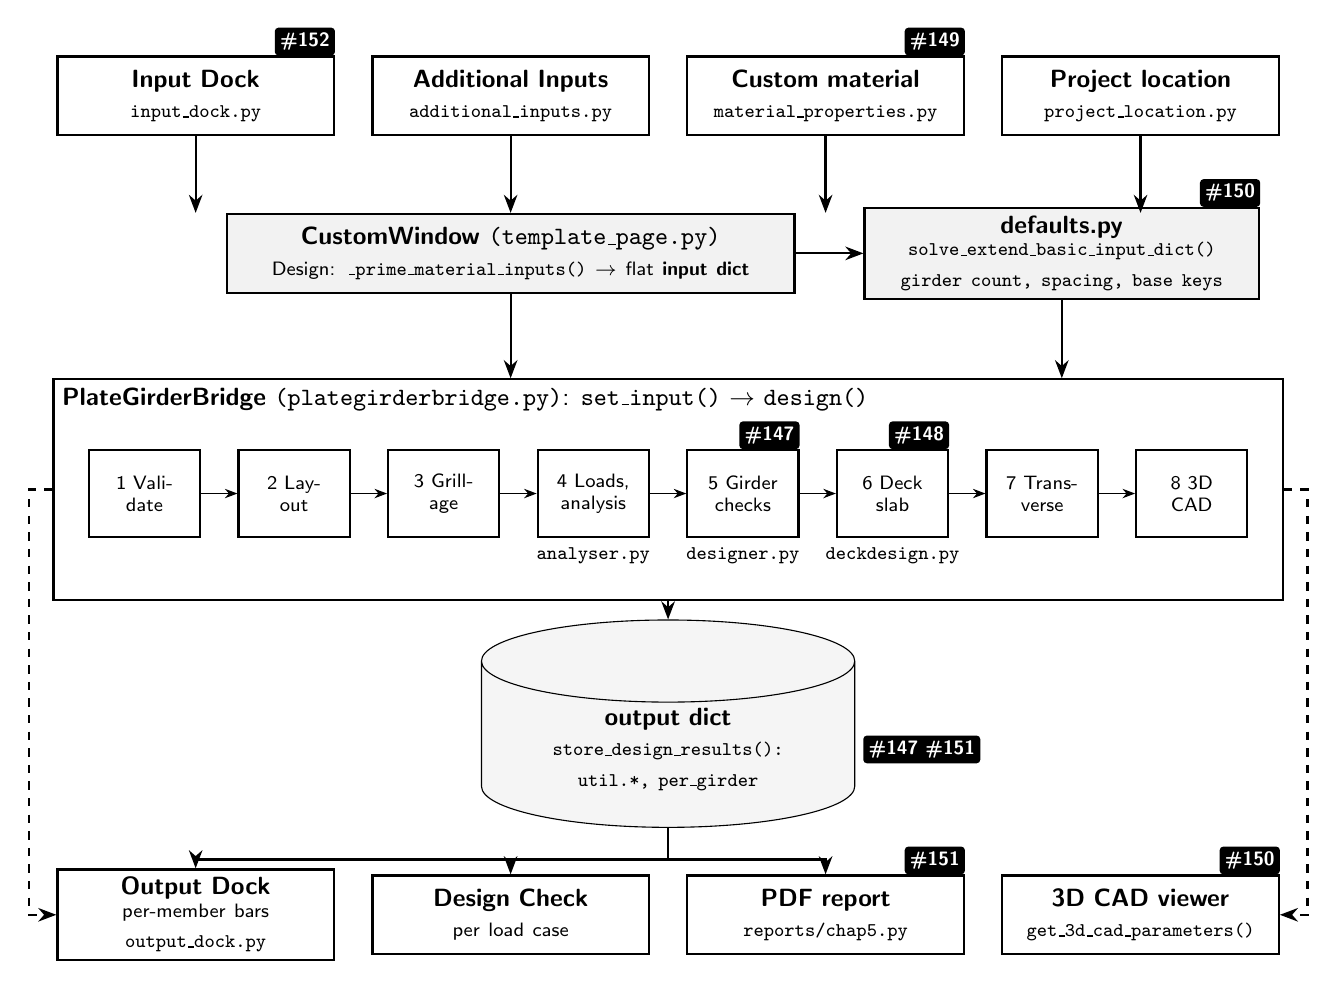
\begin{tikzpicture}[x=1cm,y=1cm]
  % --- GUI inputs
  \node[box,text width=33mm] (dock) at (-6.0,0) {\textbf{Input Dock}\\\scriptsize\ttfamily input\_dock.py};
  \node[box,text width=33mm] (add) at (-2.0,0) {\textbf{Additional Inputs}\\\scriptsize\ttfamily additional\_inputs.py};
  \node[box,text width=33mm] (mat) at (2.0,0) {\textbf{Custom material}\\\scriptsize\ttfamily material\_properties.py};
  \node[box,text width=33mm] (loc) at (6.0,0) {\textbf{Project location}\\\scriptsize\ttfamily project\_location.py};
  \node[bug,anchor=south east] at (dock.north east) {\#152};
  \node[bug,anchor=south east] at (mat.north east) {\#149};
  % --- window and defaults
  \node[gbox,text width=70mm] (win) at (-2.0,-2.0) {\textbf{CustomWindow} \texttt{(template\_page.py)}\\\scriptsize Design: \texttt{\_prime\_material\_inputs()} $\rightarrow$ flat \textbf{input dict}};
  \node[gbox,text width=48mm] (def) at (5.0,-2.0) {\textbf{defaults.py}\\\scriptsize\ttfamily solve\_extend\_basic\_input\_dict()\\ girder count, spacing, base keys};
  \node[bug,anchor=south east] at (def.north east) {\#150};
  % --- backend
  \node[box,text width=154mm,minimum height=28mm] (pgb) at (0,-5.0) {};
  \node[font=\small\sffamily,anchor=north west] at (pgb.north west) {\textbf{PlateGirderBridge}\ \texttt{(plategirderbridge.py)}: \texttt{set\_input()} $\rightarrow$ \texttt{design()}};
  \foreach \i/\t/\x in {1/{1 Vali-\\date}/-6.65,2/{2 Lay-\\out}/-4.75,3/{3 Grill-\\age}/-2.85,4/{4 Loads,\\analysis}/-0.95,5/{5 Girder\\checks}/0.95,6/{6 Deck\\slab}/2.85,7/{7 Trans-\\verse}/4.75,8/{8 3D\\CAD}/6.65}
    \node[box,text width=12mm,minimum height=11mm,font=\scriptsize\sffamily] (st\i) at (\x,-5.05) {\t};
  \foreach \a/\b in {1/2,2/3,3/4,4/5,5/6,6/7,7/8} \draw[-{Stealth[length=1.6mm]}] (st\a) -- (st\b);
  \node[font=\scriptsize\sffamily,anchor=north] at (st4.south) {\texttt{analyser.py}};
  \node[font=\scriptsize\sffamily,anchor=north] at (st5.south) {\texttt{designer.py}};
  \node[font=\scriptsize\sffamily,anchor=north] at (st6.south) {\texttt{deckdesign.py}};
  \node[bug,anchor=south east] at (st5.north east) {\#147};
  \node[bug,anchor=south east] at (st6.north east) {\#148};
  % --- output dict
  \node[store,text width=46mm] (out) at (0,-8.3) {\textbf{output dict}\\\scriptsize\ttfamily store\_design\_results(): util.*, per\_girder};
  \node[bug,anchor=west] at ($(out.east)+(1mm,0)$) {\#147 \#151};
  % --- consumers
  \node[box,text width=33mm] (od) at (-6.0,-10.4) {\textbf{Output Dock}\\\scriptsize per-member bars\\\ttfamily output\_dock.py};
  \node[box,text width=33mm] (dc) at (-2.0,-10.4) {\textbf{Design Check}\\\scriptsize per load case};
  \node[box,text width=33mm] (rep) at (2.0,-10.4) {\textbf{PDF report}\\\scriptsize\ttfamily reports/chap5.py};
  \node[box,text width=33mm] (cad) at (6.0,-10.4) {\textbf{3D CAD viewer}\\\scriptsize\ttfamily get\_3d\_cad\_parameters()};
  \node[bug,anchor=south east] at (rep.north east) {\#151};
  \node[bug,anchor=south east] at (cad.north east) {\#150};
  % --- edges
  \foreach \n in {dock,add,mat,loc} \draw[arr] (\n.south) -- (\n.south |- win.north);
  \draw[arr] (win.east) -- (def.west);
  \draw[arr] (win.south) -- (win.south |- pgb.north);
  \draw[arr] (def.south) -- (def.south |- pgb.north);
  \draw[arr] (pgb.south) -- (out.north);
  \draw[arr] (out.south) -- ++(0,-0.4) -| (rep.north);
  \draw[arr] (out.south) -- ++(0,-0.4) -| (od.north);
  \draw[arr] (out.south) -- ++(0,-0.4) -| (dc.north);
  \draw[darr] (pgb.east) -- ++(0.3,0) |- (cad.east);
  \draw[darr] (pgb.west) -- ++(-0.3,0) |- (od.west);
\end{tikzpicture}
\caption{Data flow through the plate girder module, with the location of each reported defect. Solid arrows: data saved in
the dictionaries; dashed arrows: values read directly from the back end. The Output Dock and Design Check read per-load-case
results, while the output dictionary and report read the envelope; that is why \issue{147} shows only in the report.}\label{fig:sut}
\end{figure}

\subsection{Modules examined}
\begin{table}[htbp]
\caption{Source files I read and traced while locating root causes (lines of code at \texttt{d74f56d}).}\label{tab:srcfiles}
\footnotesize
\begin{tabularx}{\linewidth}{@{}lrY@{}}
\toprule
\textbf{File} & \textbf{Lines} & \textbf{Role} \\
\midrule
\src{core/bridge\_types/plate\_girder/plategirderbridge.py} & 4\,342 & Back-end façade: \texttt{set\_input}, the 8-stage \texttt{design()}, deck call, CAD DTO, \texttt{store\_design\_results} \\
\src{core/bridge\_types/plate\_girder/designer.py} & 3\,625 & IRC 22 / IS 800 girder checks, demand extraction, fatigue range, controlling girder \\
\src{core/bridge\_types/plate\_girder/analyser.py} & 2\,869 & Grillage loads and analysis (dead, live, wind, temperature, seismic) \\
\src{core/bridge\_types/plate\_girder/deckdesign.py} & 1\,110 & Deck slab ULS/SLS design, cracked section, crack width \\
\src{core/bridge\_types/plate\_girder/defaults.py} & 939 & Derived layout keys, initial sizing, base and per-girder keys \\
\src{core/reports/chap5.py} & 1\,505 & Report Chapter 5: per-girder design tables \\
\src{desktop/ui/template\_page.py} & 2\,011 & \texttt{CustomWindow}: Design, Unlock, input-dict assembly \\
\src{desktop/ui/docks/input\_dock.py} & 1\,094 & Basic inputs, footpath handler, custom material store \\
\src{desktop/ui/dialogs/material\_properties.py} & 782 & Custom material dialog and naming \\
\bottomrule
\end{tabularx}
\end{table}

\section{Environment and setup}
I followed the given steps: fork, clone, \texttt{git checkout dev}, \texttt{conda env create -f environment.yml},
\texttt{conda activate osdagbridge-env} and \texttt{python -m osdagbridge.desktop}. Three points came up:
\begin{itemize}
\item With a fresh Miniconda 26.9, \texttt{conda env create} stops with \texttt{CondaToSNonInteractiveError}, because the terms of
  service of the Anaconda \texttt{defaults} channels have not been accepted. \texttt{environment.yml} does not need those
  channels; a \texttt{.condarc} listing only \texttt{conda-forge} (or \texttt{conda tos accept}) resolves it. A README note would help.
\item \texttt{fiona} prints \texttt{Cannot find header.dxf (GDAL\_DATA is not defined)} on import. This is harmless.
\item The loading popup starts a \texttt{multiprocessing} child. Any script that embeds the window, such as a test harness,
  must run under \texttt{if \_\_name\_\_ == "\_\_main\_\_":}, or Python raises \texttt{RuntimeError} at the first Design.
\end{itemize}

\begin{figure}[htbp]\centering
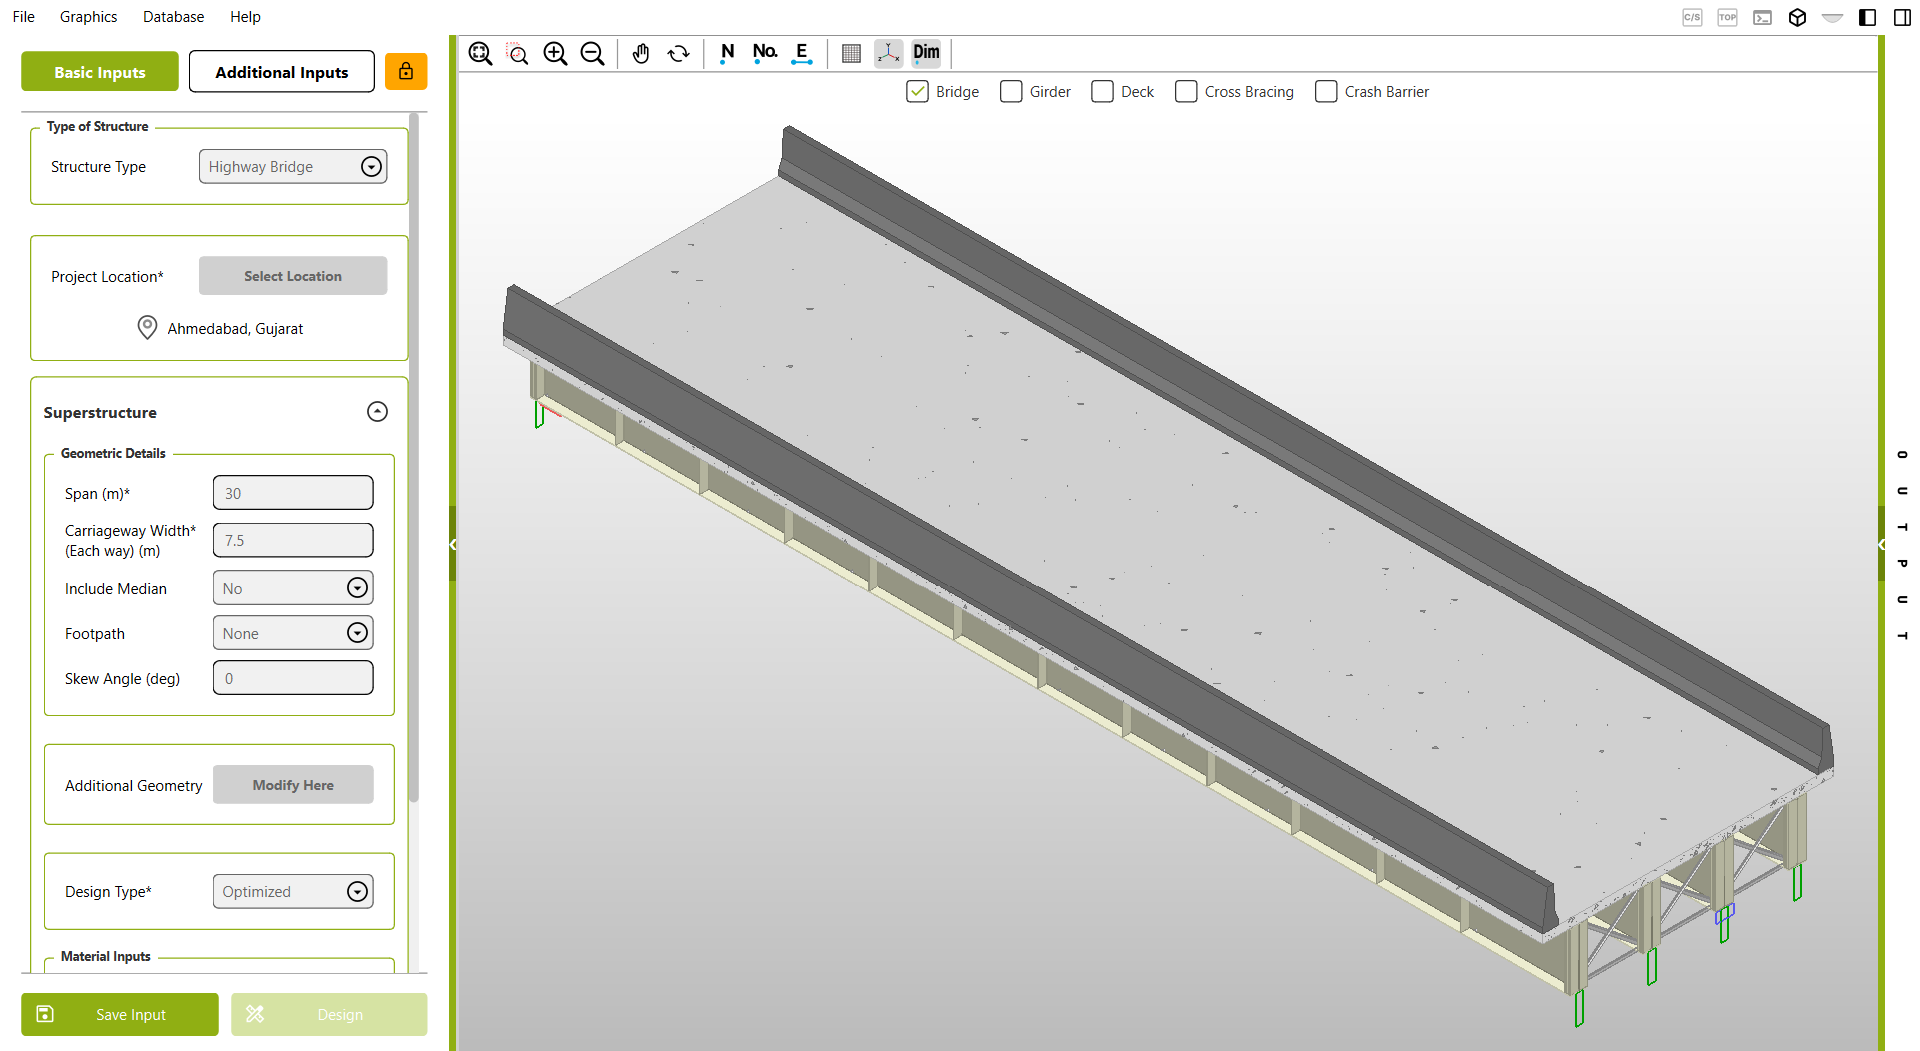
\includegraphics[width=\linewidth]{S1/TC01/window.png}
\caption{The application after the first design run (TC01: Ahmedabad, span 30 m, carriageway 7.5 m, defaults). Input Dock on
the left, 3D CAD model in the centre.}\label{fig:window}
\end{figure}

\section{Test methodology}\label{sec:method}
\subsection{Test harness architecture}
Manual clicking cannot record the dictionaries, and it is error-prone across 20 cases. I therefore wrote a small harness
(1\,354 lines in \ev{.}) that drives the real GUI through its widgets and records evidence after each run. It changes no
application code. Figure~\ref{fig:harness} shows its structure.

\begin{figure}[htbp]\centering
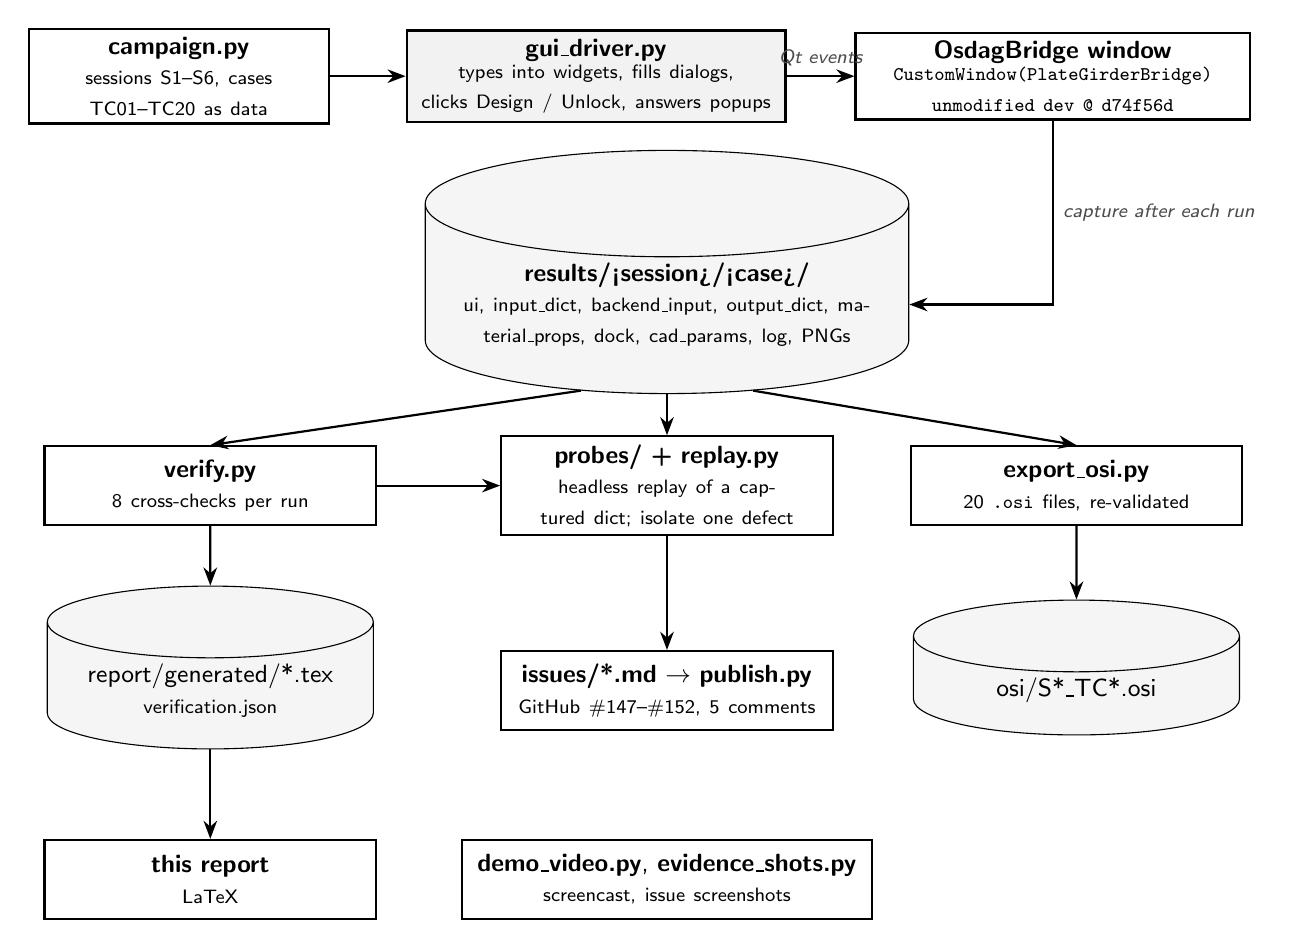
\begin{tikzpicture}[x=1cm,y=1cm]
  \node[box,text width=36mm] (camp) at (-5.6,0) {\textbf{campaign.py}\\\scriptsize sessions S1--S6, cases TC01--TC20 as data};
  \node[gbox,text width=46mm] (drv) at (-0.3,0) {\textbf{gui\_driver.py}\\\scriptsize types into widgets, fills dialogs,\\ clicks Design / Unlock, answers popups};
  \node[box,text width=48mm] (app) at (5.5,0) {\textbf{OsdagBridge window}\\\scriptsize\ttfamily CustomWindow(PlateGirderBridge)\\\scriptsize unmodified \texttt{dev} @ d74f56d};
  \node[store,text width=60mm] (res) at (0.6,-2.9) {\textbf{results/<session>/<case>/}\\\scriptsize ui, input\_dict, backend\_input, output\_dict, material\_props, dock, cad\_params, log, PNGs};
  \node[box,text width=40mm] (ver) at (-5.2,-5.2) {\textbf{verify.py}\\\scriptsize 8 cross-checks per run};
  \node[box,text width=40mm] (probe) at (0.6,-5.2) {\textbf{probes/ + replay.py}\\\scriptsize headless replay of a captured dict; isolate one defect};
  \node[box,text width=40mm] (osi) at (5.8,-5.2) {\textbf{export\_osi.py}\\\scriptsize 20 \texttt{.osi} files, re-validated};
  \node[store,text width=40mm] (gen) at (-5.2,-7.8) {report/generated/*.tex\\\scriptsize verification.json};
  \node[box,text width=40mm] (iss) at (0.6,-7.8) {\textbf{issues/*.md} $\rightarrow$ \textbf{publish.py}\\\scriptsize GitHub \#147--\#152, 5 comments};
  \node[store,text width=40mm] (osif) at (5.8,-7.8) {osi/S*\_TC*.osi};
  \node[box,text width=40mm] (rep) at (-5.2,-10.2) {\textbf{this report}\\\scriptsize LaTeX};
  \node[box,text width=50mm] (vid) at (0.6,-10.2) {\textbf{demo\_video.py}, \textbf{evidence\_shots.py}\\\scriptsize screencast, issue screenshots};
  \draw[arr] (camp) -- (drv);
  \draw[arr] (drv) -- node[lbl,above]{Qt events} (app);
  \draw[arr] (app.south) |- node[lbl,pos=0.25,right]{capture after each run} (res.east);
  \draw[arr] (res.south west) -- (ver.north);
  \draw[arr] (res.south) -- (probe.north);
  \draw[arr] (res.south east) -- (osi.north);
  \draw[arr] (ver) -- (gen);
  \draw[arr] (probe) -- (iss);
  \draw[arr] (osi) -- (osif);
  \draw[arr] (gen) -- (rep);
  \draw[arr] (ver.east) -- (probe.west);
\end{tikzpicture}
\caption{Test harness. The GUI is driven through the same widgets, signals, validators and dialogs a user operates; the design
runs on the application's own worker thread.}\label{fig:harness}
\end{figure}

\begin{table}[htbp]
\caption{Evidence captured for every case in \texttt{results/<session>/<case>/}.}\label{tab:evidence}
\footnotesize
\begin{tabularx}{\linewidth}{@{}lY@{}}
\toprule
\textbf{File} & \textbf{Content} \\
\midrule
\texttt{ui.json} & Every widget value in the Input Dock and the dialogs, as displayed \\
\texttt{input\_dict.json} & The dictionary Design hands to \texttt{set\_input()} \\
\texttt{backend\_input.json} & \texttt{PlateGirderBridge.input\_dict} after \texttt{design()} (unit conversions applied) \\
\texttt{output\_dict.json} & The output dictionary used by the report \\
\texttt{material\_props.json} & \texttt{steel\_prop} and \texttt{concrete\_prop} objects the analysis actually used \\
\texttt{dock.json} & Every Output Dock bar for every member and load case, including \emph{Design Envelope} \\
\texttt{cad\_params.json}, \texttt{cad\_info\_table.json} & The DTO passed to the 3D viewer and its info table \\
\texttt{meta.json}, \texttt{log.txt} & Actions taken, popups answered, timings; the log dock \\
\texttt{window.png}, \texttt{cad3d.png}, \texttt{plots.png}, \texttt{cross\_section.png}, \texttt{top\_view.png} & Screenshots \\
\bottomrule
\end{tabularx}
\end{table}

\subsection{Cross-checks}
\texttt{verify.py} runs eight checks on every run and writes the tables used in this report: (1) UI value vs input dict vs
backend input vs output dict; (2) material values typed vs the properties the analysis used; (3) \texttt{util.*} vs the worst
Output Dock bar; (4) CAD DTO vs the designed girder and bracing; (5) girder layout vs a fresh session with the same inputs;
(6) image outputs vs the previous run (checksums); (7) report tables vs \texttt{per\_girder}; (8) \texttt{.osi} round trip.
When a check failed, a \emph{probe} replayed the captured input dictionary headless and isolated the defect to a line of code.

\subsection{Test design and component coverage}
Sessions were designed so that each one exercises one area and runs its cases back to back in a single window, which also
tests state persistence. S5 and S6 are controls that separate genuine carry-over from intended behaviour.
\begin{table}[htbp]
\caption{Component coverage by session ($\bullet$ = custom or non-default values entered and verified; $\circ$ = default values verified).}\label{tab:coverage}
\small
\begin{tabular}{@{}lcccccc@{}}
\toprule
\textbf{Component} & \textbf{S1} & \textbf{S2} & \textbf{S3} & \textbf{S4} & \textbf{S5} & \textbf{S6} \\
\midrule
Girders (database grades E 250A--E 410A) & $\bullet$ & $\bullet$ & $\circ$ & & $\circ$ & $\circ$ \\
Girders (custom steel) & & $\bullet$ & & $\bullet$ & & \\
Girder section, unsymmetric (Custom mode) & & & $\bullet$ & & & \\
Intermediate and bearing stiffeners & $\circ$ & $\circ$ & $\bullet$ & & $\circ$ & $\circ$ \\
Cross bracing (database / custom steel) & $\bullet$ & $\bullet$ & $\circ$ & & $\circ$ & $\circ$ \\
End diaphragm (database / custom steel) & $\bullet$ & $\bullet$ & $\circ$ & & $\circ$ & $\circ$ \\
Shear studs (diameter, height) & $\circ$ & $\circ$ & $\bullet$ & & $\circ$ & $\circ$ \\
Deck slab: concrete (M30, M35, custom) & $\bullet$ & $\bullet$ & $\circ$ & & $\circ$ & $\circ$ \\
Deck slab: thickness, cover, reinforcement & $\circ$ & $\circ$ & $\bullet$ & & $\circ$ & $\circ$ \\
Geometry: span, carriageway, skew, median, footpath & $\bullet$ & $\bullet$ & $\bullet$ & $\bullet$ & $\bullet$ & $\bullet$ \\
Input validation & & & & $\bullet$ & & \\
\bottomrule
\end{tabular}
\end{table}

\section{Test cases}\label{sec:cases}
Table~\ref{tab:cases} lists every case with its inputs in the order they were entered. Cases after the first in a session start
from the previous run's state. ``\#147'' etc.\ mark defects found in that run; ``(expected)'' marks behaviour that matches the
specification. Abbreviations: cw = carriageway width (each way), CB = cross bracing, ED = end diaphragm, rho = density,
alpha = thermal coefficient. In total: \textbf{15 design runs completed} (all with at least one defect from
Table~\ref{tab:outcome}), \textbf{5 validation cases passed}.
\clearpage
{\footnotesize\setlength{\tabcolsep}{3pt}\begin{longtable}{@{}L{0.06\textwidth}L{0.42\textwidth}L{0.19\textwidth}L{0.27\textwidth}@{}}
\caption{Test cases: exact inputs in entry order, outcome of the run and findings.}\label{tab:cases}\\
\toprule
\textbf{Case} & \textbf{Exact inputs (in entry order)} & \textbf{Run} & \textbf{Findings} \\
\midrule\endfirsthead
\toprule
\textbf{Case} & \textbf{Exact inputs (in entry order)} & \textbf{Run} & \textbf{Findings} \\
\midrule\endhead
\multicolumn{4}{@{}L{0.97\textwidth}@{}}{\textbf{S1}: Basic geometry sweep with database grades, 4 consecutive runs (Ahmedabad, Gujarat)} \\*
TC01 & span 30, cw 7.5, skew 0 & designed: 4 girders at 2.1 m & \#148 deck SLS; \#151 report tables; \#66 Table 2.7 units; \#147 \\
TC02 & after unlock: span 40, skew 10, footpath Single Side & designed: 4 girders at 2.569 m & \#147; \#112 (fresh: 5); \#89 \\
TC03 & after unlock: cw 11, skew -12, median Yes, footpath Both Sides & designed: 4 girders at 6.963 m & 27.85 m deck on 4 girders, shear 188 \%; CAD legend width 26.45 m (\#124); \#147; \#112 (fresh: 12); \#89 \\
TC04 & after unlock: span 20, cw 7.5, skew 15, median No, footpath None, girder E 250A, CB E 300A, ED E 410A, deck M30 & designed: 4 girders at 2.1 m & span/skew limits 20 m / 15 deg accepted; \#147; \#89 \\
\multicolumn{4}{@{}L{0.97\textwidth}@{}}{\textbf{S2}: Custom materials for girder, cross bracing, end diaphragm and deck, 4 consecutive runs (Chennai (Minambakkam) (A), Tamil Nadu)} \\*
TC05 & span 25, cw 7.5, skew 5, girder custom (rho 78.5, Fy 345, Fu 480, E 205, nu 0.3, alpha 12.0), CB custom (rho 77.0, Fy 260, Fu 410, E 200, nu 0.3, alpha 11.7), ED custom (rho 76.9, Fy 300, Fu 440, E 200, nu 0.3, alpha 11.7), deck custom (rho 25.5, fck 42, fctm 3.2, Ecm 33.5, alpha 10.5) & designed: 4 girders at 2.1 m & custom Fy/Fu/E reach analysis; densities not used (\#20, \#41); CB/ED grades unused (\#43); \#147; \#89 \\
TC06 & after unlock: deck M35, girder custom (rho 80.0, Fy 410, Fu 540, E 210, nu 0.3, alpha 12.0) & designed: 4 girders at 2.1 m & density 80 ignored (\#20); \#147; \#89 \\
TC07 & after unlock: girder E 350A & designed: 4 girders at 2.1 m & custom to database grade: OK; \#147; \#89 \\
TC08 & after unlock: girder custom\_steel\_410\_540, CB custom (rho 77.0, Fy 410, Fu 540, E 200, nu 0.3, alpha 11.7) & designed: 4 girders at 2.1 m & name collision: girder E 210 to 200, rho 80 to 77 (\#149); \#147; \#89 \\
\multicolumn{4}{@{}L{0.97\textwidth}@{}}{\textbf{S3}: Custom design mode, custom girder section, stiffeners, deck and stud inputs, 3 runs (Guwahati (Bhorjar) (A), Assam)} \\*
TC09 & span 35, cw 9, skew 0, mode Custom, symmetry Girder Unsymmetric, depth 1800, top flange width 450, top flange thickness 25, bottom flange width 550, bottom flange thickness 32, web thickness 14, intermediate stiffener Yes, intermediate stiffener spacing 1800, intermediate stiffener thickness 12, intermediate stiffener outstand 150, bearing stiffener plate thickness 16, bearing stiffener outstand 200, deck thickness 230, thickness 65, diameter 22, height 120, bottom clear cover 40 & designed: 4 girders at 2.475 m & custom section, stiffeners, deck, studs reach design and CAD; \#148, \#151; \#147 \\
TC10 & after unlock: depth 1600, deck thickness 260, intermediate stiffener spacing 1500 & designed: 4 girders at 2.475 m & Additional Inputs survive unlock; design and CAD agree; \#147 \\
TC11 & after unlock: span 38 & designed: 4 girders at 2.475 m & deck 260 to 250, stud 22 to 20, cover 40 to 50 (\#71); CAD draws 2120 mm girder (\#150); \#147 \\
\multicolumn{4}{@{}L{0.97\textwidth}@{}}{\textbf{S4}: Input validation (no design runs)} \\*
TC12 & nothing entered & no design: Empty Required Fields & blocked, empty fields listed (expected) \\
TC13 & typed span 19, typed span 46 & 19 shown as 20.0; 46 shown as 45.0 & clamped with warning (expected) \\
TC14 & typed cw 4.0, typed cw 24, median Yes, typed cw 7.0 & 4.0 shown as 4.25; 24 shown as 23.6; 7.0 shown as 7.5 & clamped with warning (expected) \\
TC15 & typed skew 20, typed skew -20 & 20 shown as 15.0; -20 shown as -15.0 & clamped with warning (expected) \\
TC16 & girder custom (rho 30, Fy 1300, Fu 1400, E 200, nu 0.3, alpha 11.7) & saved as custom\_steel\_1200\_1400 after 2 range warnings & clamped with warning (expected) \\
\multicolumn{4}{@{}L{0.97\textwidth}@{}}{\textbf{S5}: Control: girder layout when the deck width changes between runs (Ahmedabad, Gujarat)} \\*
TC17 & span 40, cw 11, skew -12, median Yes, footpath Both Sides & designed: 5 girders at 5.57 m & \#147; \#112 (fresh: 12); \#89 \\
TC18 & after unlock: span 30, cw 7.5, skew 0, median No, footpath None & designed: 5 girders at 1.68 m & \#147; \#112 (fresh: 4) \\
\multicolumn{4}{@{}L{0.97\textwidth}@{}}{\textbf{S6}: Control: girder count seeded on a wide deck, then the deck is narrowed (Ahmedabad, Gujarat)} \\*
TC19 & median Yes, footpath Both Sides, span 40, cw 11, skew 0 & designed: 7 girders at 3.979 m & live load dropped, all demands 0, PASS (\#134); util 0.0 (\#45); \#112 (fresh: 12) \\
TC20 & after unlock: span 30, cw 7.5, median No, footpath None & designed: 7 girders at 1.2 m & \#147; \#112 (fresh: 4) \\
\bottomrule
\end{longtable}
}

\section{UI inputs versus input and output dictionaries}\label{sec:dicts}
Tables~\ref{tab:tc01} to~\ref{tab:tc09} follow single values from the UI through the dictionaries to the analysis, and
Table~\ref{tab:consistency} summarises the same checks for every run. The GUI stores girder dimensions in mm and
\texttt{design()} converts the backend copy to metres, which is why the backend columns show 1.8 for 1800.

\begin{table}[htbp]\centering
\caption{TC01: Input Dock against the three dictionaries. Layout keys are derived by \texttt{solve\_extend\_basic\_input\_dict()}.}\label{tab:tc01}
\gentab{sbs_tc01.tex}
\end{table}

\begin{table}[htbp]\centering
\caption{TC05: values typed in the custom-material dialogs against the dictionaries and \texttt{material\_props} used by the
analysis. G is derived from E and $\nu$. Every value reaches both dictionaries. The girder density shows OK only because it
equals the fixed analysis constant (78.5); densities and thermal coefficients are never read (\issue{20}, \issue{41}), and the
cross-bracing and end-diaphragm grades are not used by the design (\issue{43}).}\label{tab:tc05}
\gentab{sbs_tc05.tex}
\end{table}

\begin{table}[htbp]\centering
\caption{TC09 (Custom mode): Additional Inputs against the dictionaries, the girder designer and the 3D CAD DTO. Every value
arrives everywhere. After TC11 changes only the span, the CAD column switches to the initial-sizing girder (\issue{150}) and
deck thickness, stud size and cover revert to defaults (\issue{71}).}\label{tab:tc09}
\gentab{sbs_tc09.tex}
\end{table}

\begin{table}[htbp]\centering
\caption{Consistency per design run. ``Not used as entered'' lists material properties whose dictionary value differs from
the value the analysis applies. ``Output $\ne$ Dock'' lists categories where \texttt{util.*} differs from the worst Output Dock
bar by more than 1 point.}\label{tab:consistency}
\gentab{dict_consistency.tex}
\end{table}

\section{Output verification}\label{sec:outputs}
\subsection{Output dictionary against the Output Dock}
Table~\ref{tab:util} compares each utilisation in the output dictionary with the worst Output Dock bar. Fatigue differs by a
factor of 2.00 in all 14 runs that produce a fatigue check (\issue{147}, Section~\ref{sec:i147}). Shear and stress limitation
differ because \texttt{util.*} holds the controlling girder rather than the worst girder per category (\issue{151}). In TC19 the
live load was silently dropped and all demands were zero (\issue{134}).

\begin{table}[htbp]\centering
\caption{\texttt{util.*} in the output dictionary / worst Output Dock bar over all members, \emph{Design Envelope} (\%).}\label{tab:util}
\gentab{util.tex}
\end{table}

\begin{figure}[htbp]\centering
\begin{subfigure}[t]{0.3\linewidth}\centering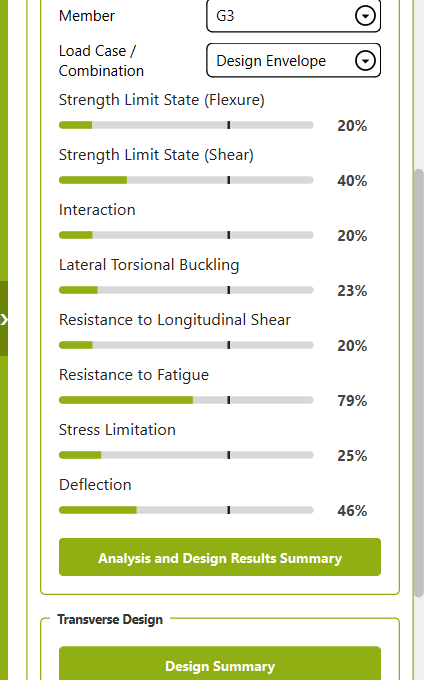
\includegraphics[height=6.4cm]{figures/dock_fatigue.png}\caption{Output Dock, G3, \emph{Design Envelope}}\end{subfigure}\hfill
\begin{subfigure}[t]{0.66\linewidth}\centering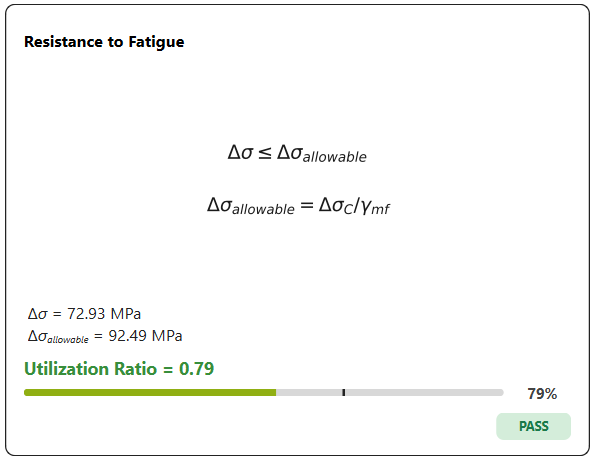
\includegraphics[height=6.4cm]{figures/design_check_fatigue.png}\caption{Design Check tab, G3, SLS\_FREQUENT\_1}\end{subfigure}\\[8pt]
\begin{subfigure}[t]{\linewidth}\centering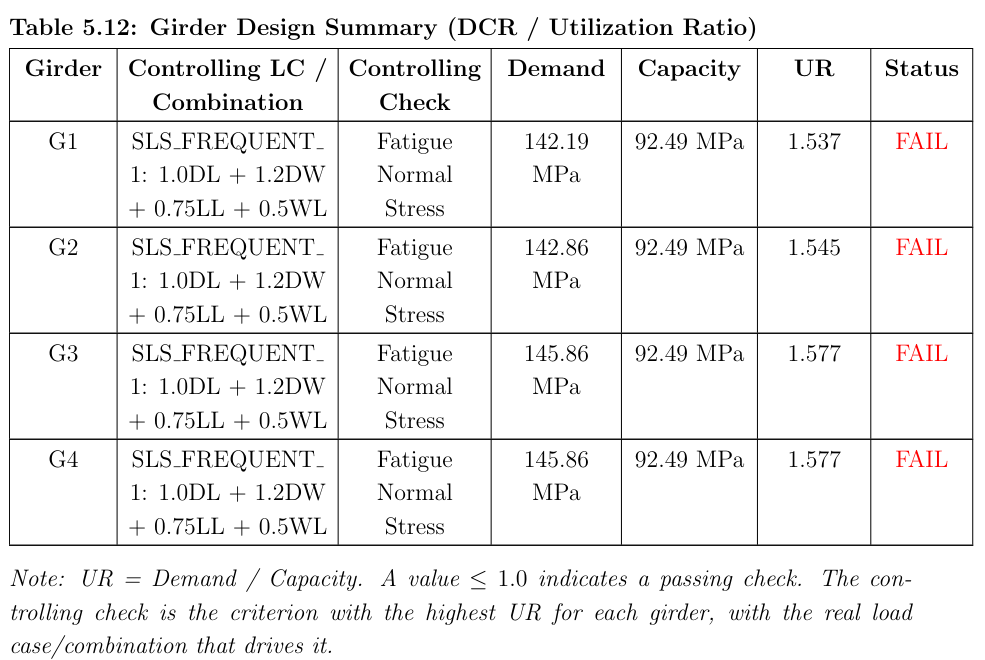
\includegraphics[width=0.62\linewidth]{figures/report_fatigue_table.png}\caption{Design report, Table 5.12}\end{subfigure}
\caption{TC01, girder G3, Fatigue Normal Stress. The GUI shows $\Delta\sigma$ = 72.93 MPa, UR 0.79, PASS. The report for the
same run shows 145.86 MPa, UR 1.577, FAIL (\issue{147}).}\label{fig:fatigue}
\end{figure}

\subsection{Output dictionary against the design report}
\begin{itemize}
\item Overall utilisation 1.58 (fatigue) in the Executive Summary and Table 5.12 equals \texttt{util.fatigue}/100, so it is doubled (\issue{147}).
\item Tables 5.1--5.6 print one value for every girder, the controlling girder's (Figure~\ref{fig:moment}). For TC01 the shear
  rows read 288.29 kN and UR 0.40, while \texttt{per\_girder} holds 379.98 kN for the exterior girders and the Output Dock shows
  53\,\% for G2 (\issue{151}). TC09 shows the same pattern: 383.37 kN printed against 517.22 kN.
\item Table 2.7 prints the girder in metres labelled mm (``1.67 mm''), confirming \issue{66}.
\item Chapter 3 states ``Steel Self-Weight Applied 76.4 kN/m\textsuperscript{3}'' while the self-weight load uses 78.5 (comment on \issue{20}).
\item Values that match: span, carriageway, girder plates (Table 5.1), material grades, deck thickness, stud dimensions, deck
  reinforcement and the deck utilisation ratios agree with \texttt{output\_dict} in both reports (deck ratios within rounding).
\end{itemize}

\begin{figure}[htbp]\centering
\begin{subfigure}[t]{0.46\linewidth}\centering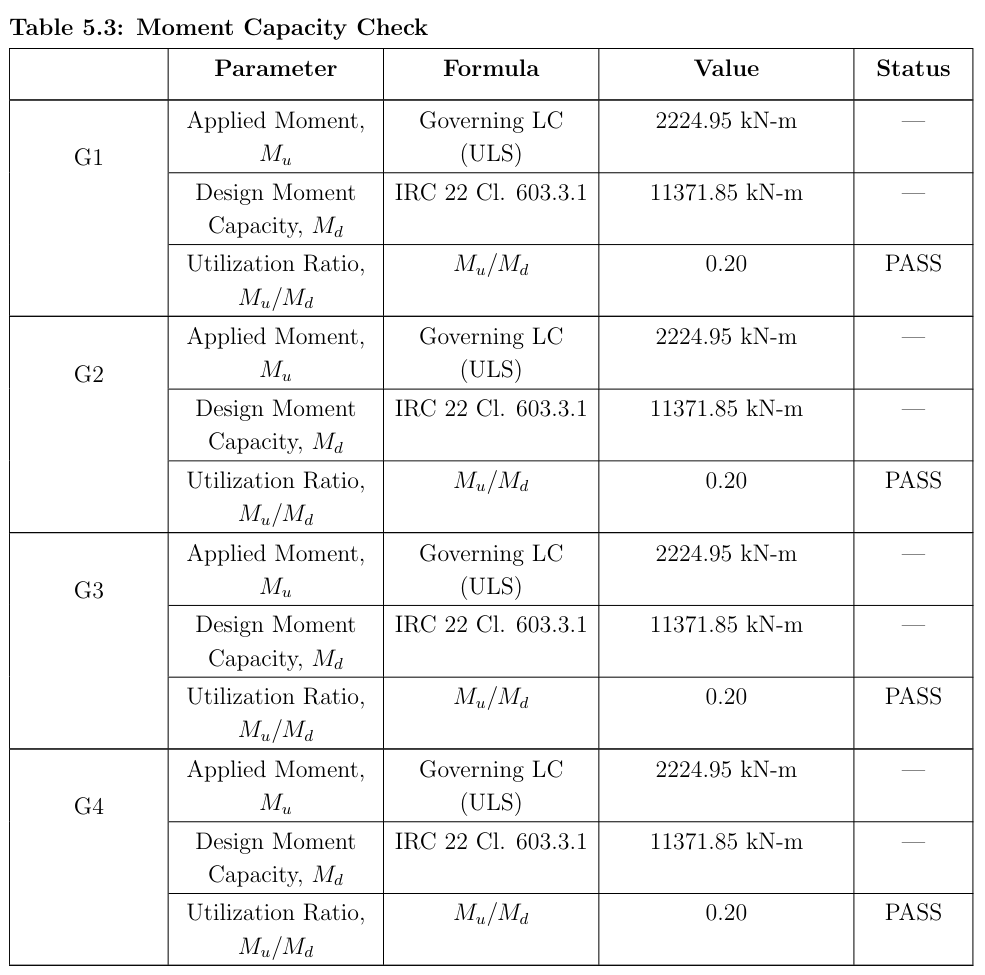
\includegraphics[width=\linewidth]{figures/report_moment_table.png}\caption{TC01 report, Table 5.3}\end{subfigure}\hfill
\begin{subfigure}[t]{0.5\linewidth}\centering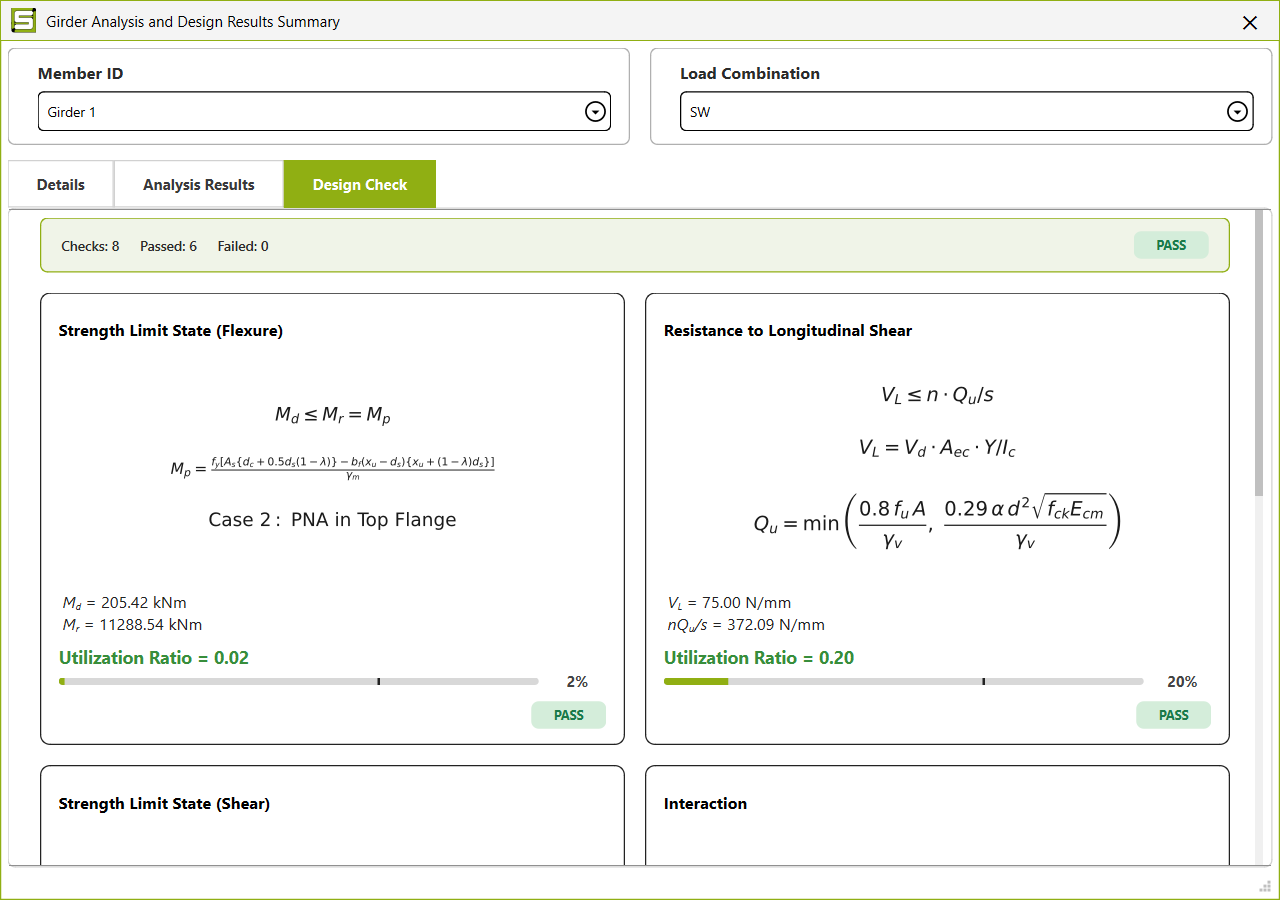
\includegraphics[width=\linewidth]{demo/steel_design_check_run1.png}\caption{Design Check for Girder 1, load combination SW}\end{subfigure}
\caption{(a) The same moment (2224.95 kN·m) and UR for every girder, the controlling girder's values; \texttt{per\_girder}
holds 2181.62 kN·m for the exterior girders (\issue{151}). (b) The per-load-case Design Check dialog, which reads the
per-girder results correctly.}\label{fig:moment}
\end{figure}

\section{Input validation}\label{sec:validation}
Session S4 entered out-of-range and missing values. All five cases behaved as specified: values are clamped to the code
limits with a warning, and Design is blocked while required fields are empty (Table~\ref{tab:cases}, TC12--TC16).
\begin{figure}[htbp]\centering
\begin{subfigure}[t]{0.32\linewidth}\centering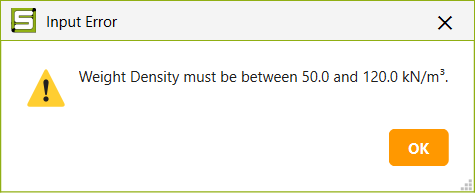
\includegraphics[width=\linewidth]{S4/popup_01.png}\caption{Custom density 30 (TC16)}\end{subfigure}\hfill
\begin{subfigure}[t]{0.32\linewidth}\centering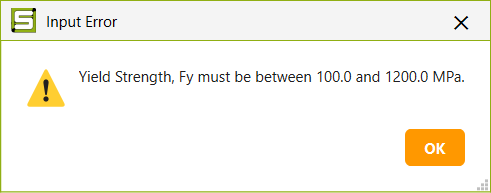
\includegraphics[width=\linewidth]{S4/popup_02.png}\caption{Custom Fy 1300 (TC16)}\end{subfigure}\hfill
\begin{subfigure}[t]{0.32\linewidth}\centering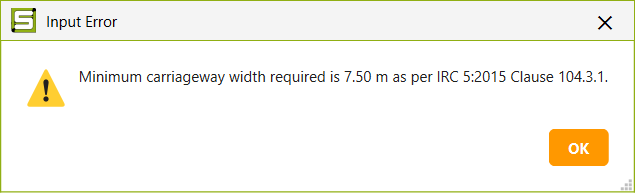
\includegraphics[width=\linewidth]{S4/popup_03.png}\caption{Carriageway 7.0 with median (TC14)}\end{subfigure}\\[6pt]
\begin{subfigure}[t]{0.32\linewidth}\centering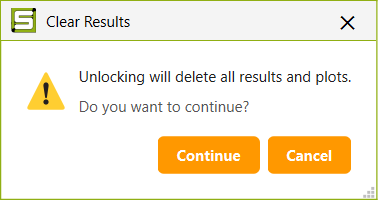
\includegraphics[width=\linewidth]{S1/popup_01.png}\caption{Unlock before a redesign}\end{subfigure}\qquad
\begin{subfigure}[t]{0.25\linewidth}\centering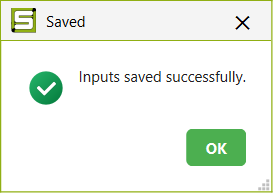
\includegraphics[width=\linewidth]{S3/popup_03.png}\caption{Additional Inputs saved}\end{subfigure}
\caption{Validation and confirmation dialogs captured during the sessions.}\label{fig:popups}
\end{figure}

\section{Multi-run stability and state persistence}\label{sec:multirun}
Table~\ref{tab:multirun} compares each run with the previous run in the same window, and Figure~\ref{fig:cad-s1} shows the
3D CAD of the four runs of session S1. The window stayed responsive and nothing crashed, but state carries over between runs
(Table~\ref{tab:layout}, Figure~\ref{fig:state}):
\begin{itemize}
\item \textbf{Girder count} is seeded once and only re-spaced afterwards (\issue{112}, extended in a comment). TC03 puts a
  27.85 m deck on 4 girders at 6.96 m with 3.48 m overhangs (shear 188\,\%), where a fresh session gives 12 girders. TC20 keeps 7
  girders at 1.20 m on an 8.4 m deck (fresh: 4). Skewed runs keep only one girder line (\issue{89}).
\item \textbf{Additional Inputs} (deck 260 mm, stud 22 mm, cover 40 mm) reverted to defaults when only the span changed (TC11, \issue{71}).
\item \textbf{Custom-mode girder}: after the span change the base keys hold the initial-sizing girder, so the CAD draws 2120 mm
  while the check uses 1600 mm (\issue{150}).
\item \textbf{Custom materials}: re-selecting a stored custom grade restores its values (TC07 to TC08), but creating a second
  custom steel with the same Fy/Fu overwrote the girder's E and density (\issue{149}).
\end{itemize}

\begin{table}[htbp]\centering
\caption{Consecutive runs in one window (unlock, edit, Design). Image outputs are compared by checksum with the previous run.
* Unchanged because only material grades changed, which is expected.}\label{tab:multirun}
\gentab{multirun.tex}
\end{table}

\begin{figure}[htbp]\centering
\begin{subfigure}[t]{0.24\linewidth}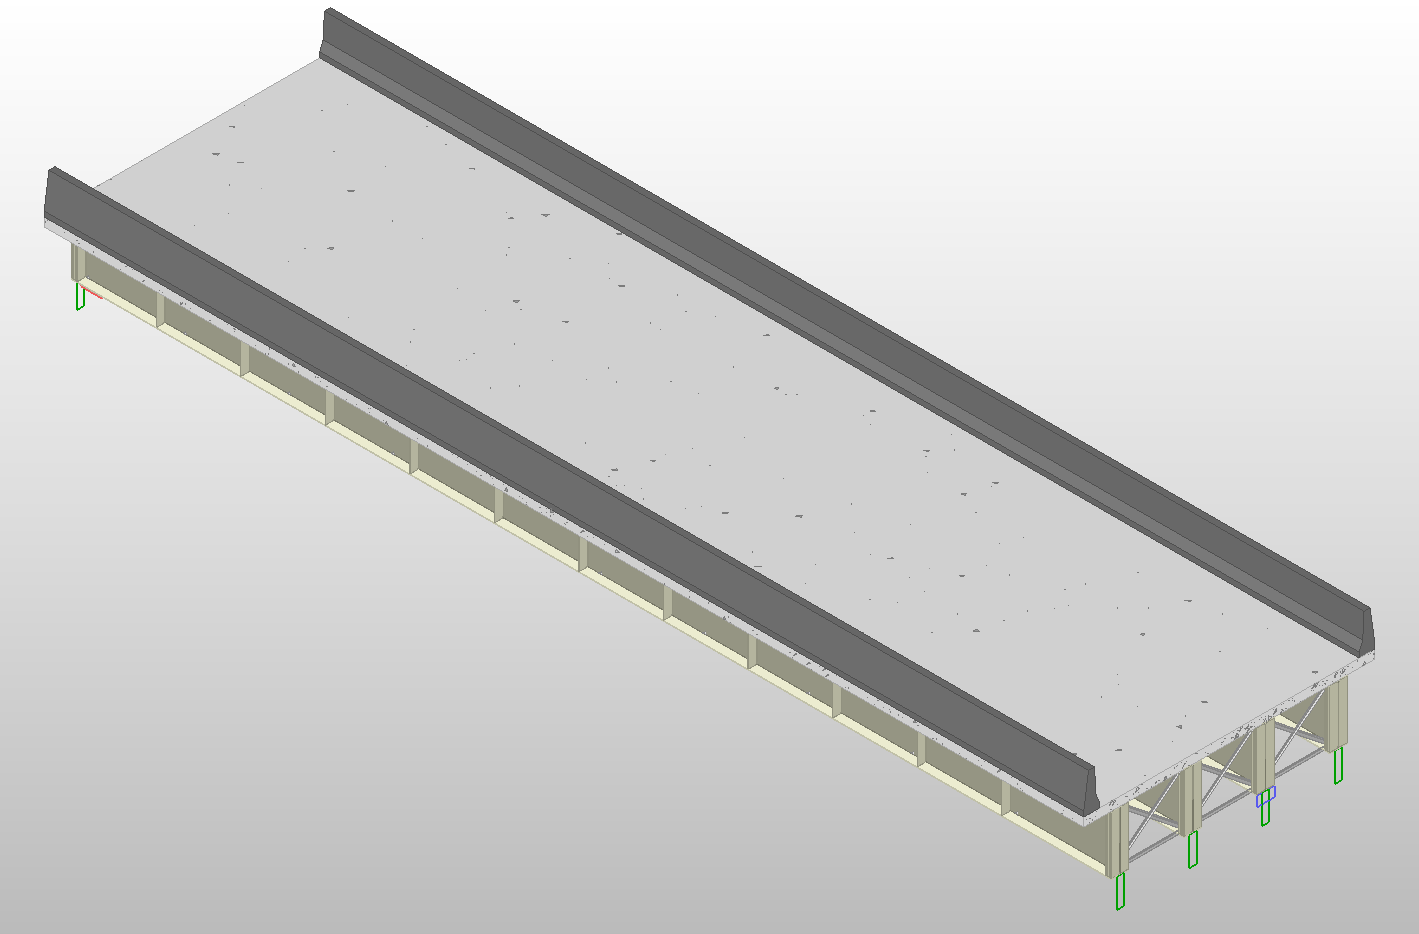
\includegraphics[width=\linewidth]{S1/TC01/cad3d.png}\caption{TC01: 30 m}\end{subfigure}\hfill
\begin{subfigure}[t]{0.24\linewidth}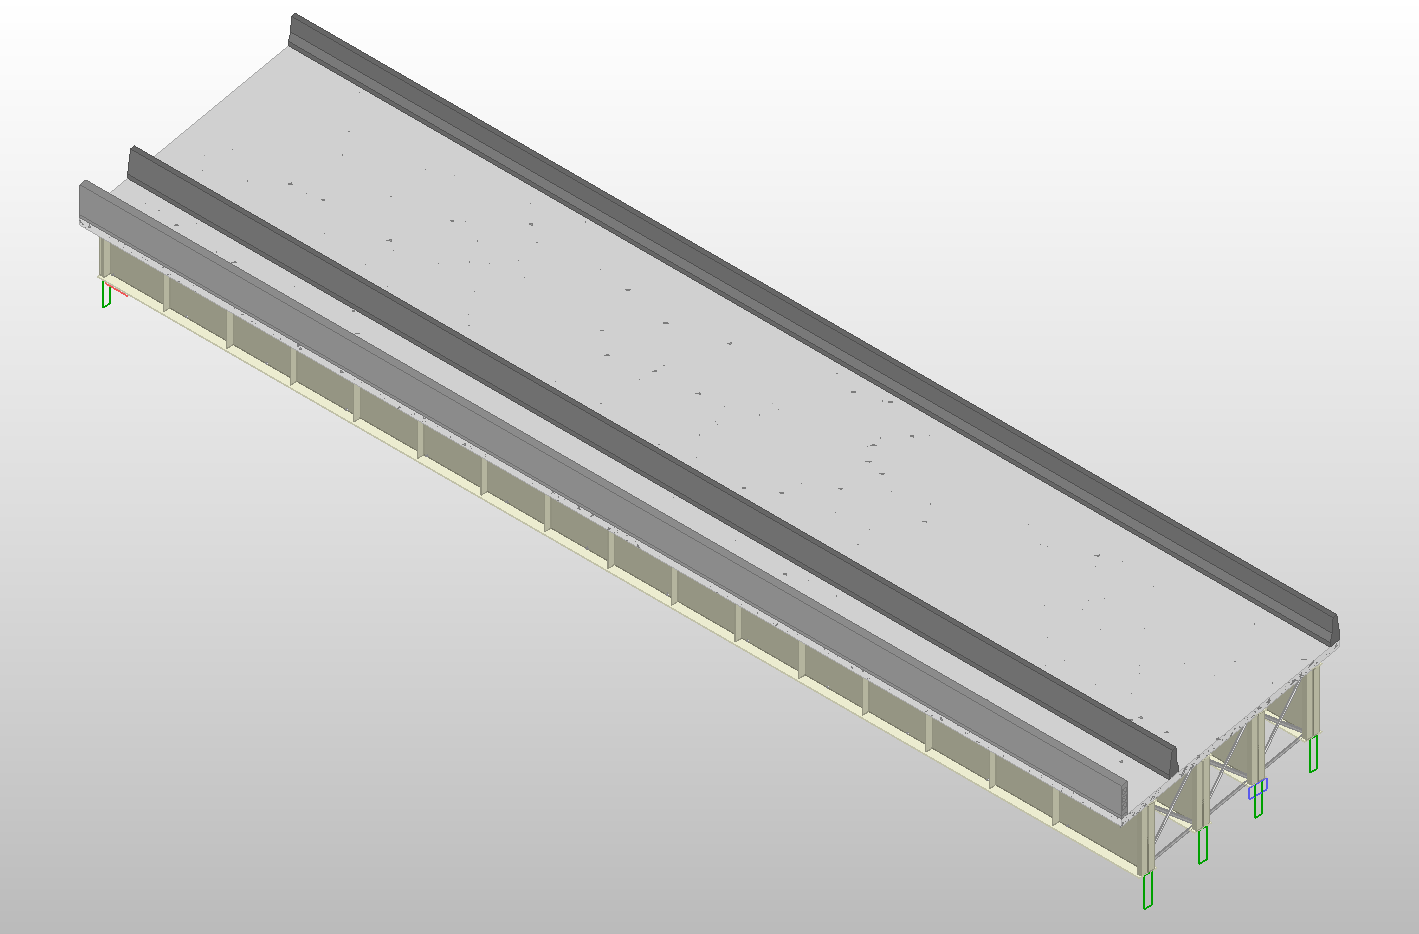
\includegraphics[width=\linewidth]{S1/TC02/cad3d.png}\caption{TC02: 40 m, footpath}\end{subfigure}\hfill
\begin{subfigure}[t]{0.24\linewidth}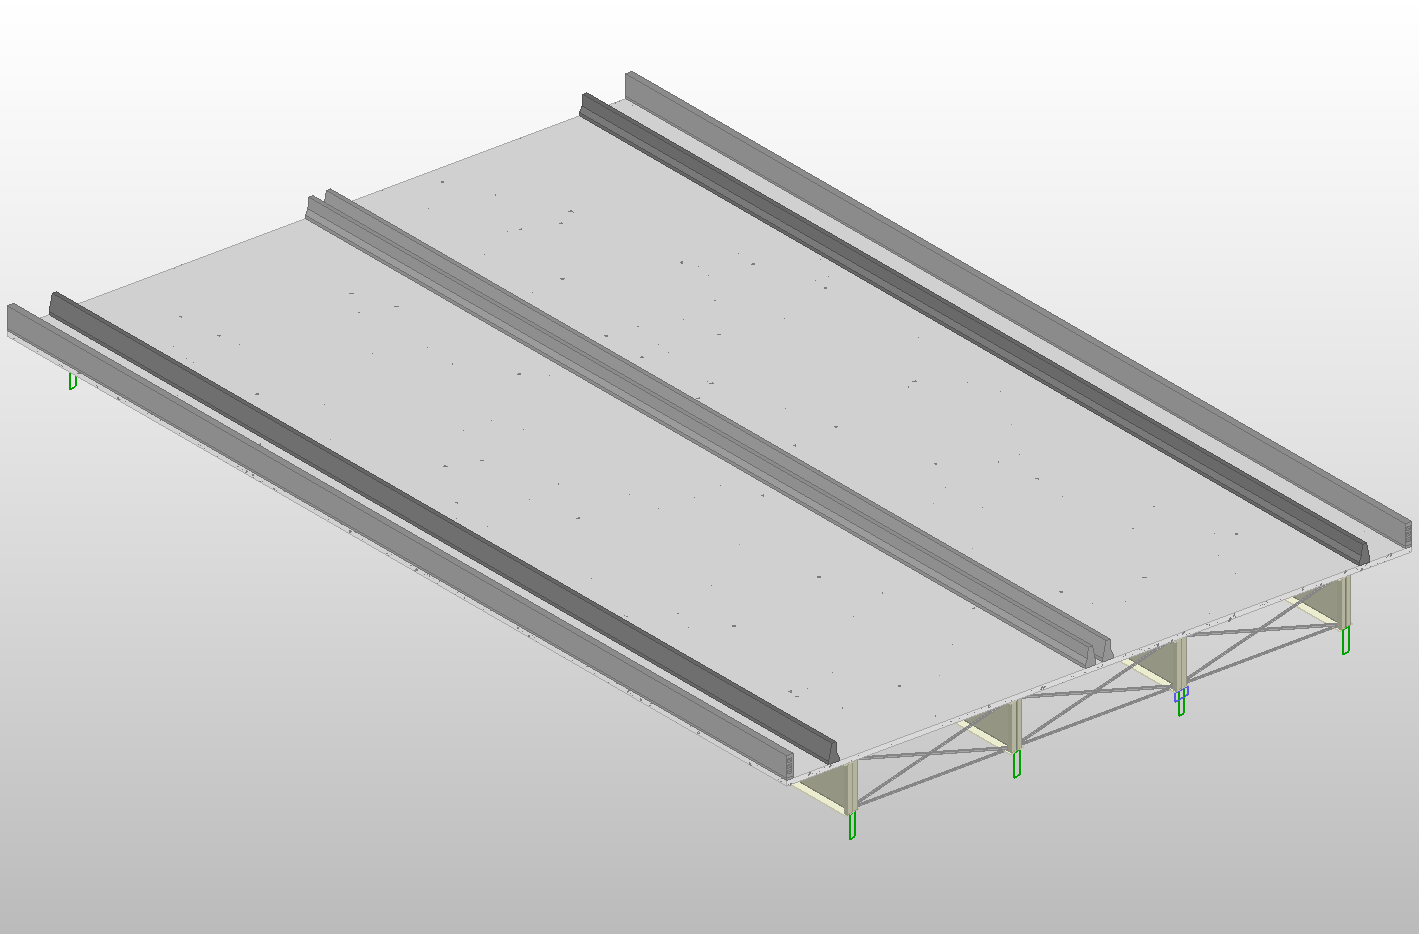
\includegraphics[width=\linewidth]{S1/TC03/cad3d.png}\caption{TC03: median, footpaths}\end{subfigure}\hfill
\begin{subfigure}[t]{0.24\linewidth}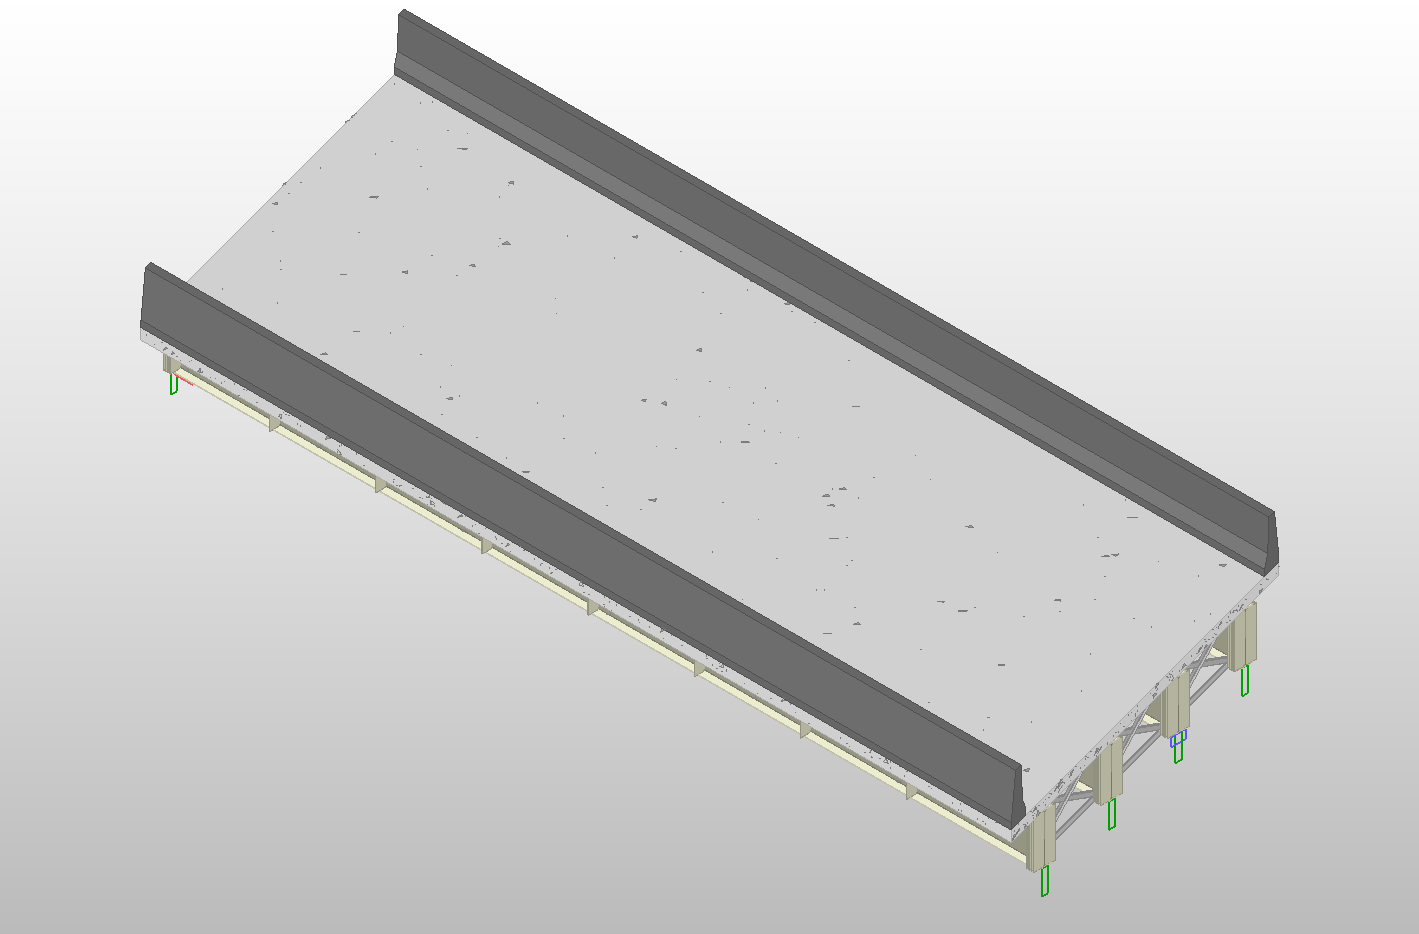
\includegraphics[width=\linewidth]{S1/TC04/cad3d.png}\caption{TC04: 20 m, skew 15}\end{subfigure}
\caption{3D CAD rebuilt on each of four consecutive runs of session S1.}\label{fig:cad-s1}
\end{figure}

\begin{table}[htbp]\centering
\caption{Girder layout per run against a fresh session given the same final homepage inputs.}\label{tab:layout}
\gentab{layout.tex}
\end{table}

\begin{figure}[htbp]\centering
\begin{subfigure}[t]{\linewidth}\centering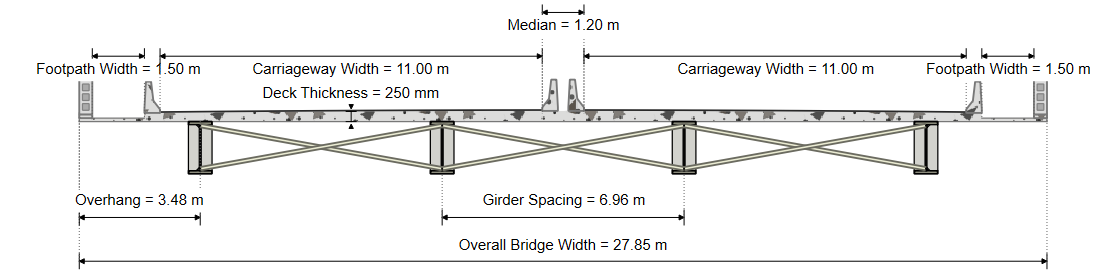
\includegraphics[width=0.92\linewidth]{figures/tc03_cross_section.png}\caption{TC03 cross-section after three consecutive runs: a 27.85 m deck on 4 girders at 6.96 m (\issue{112})}\end{subfigure}\\[8pt]
\begin{subfigure}[t]{0.48\linewidth}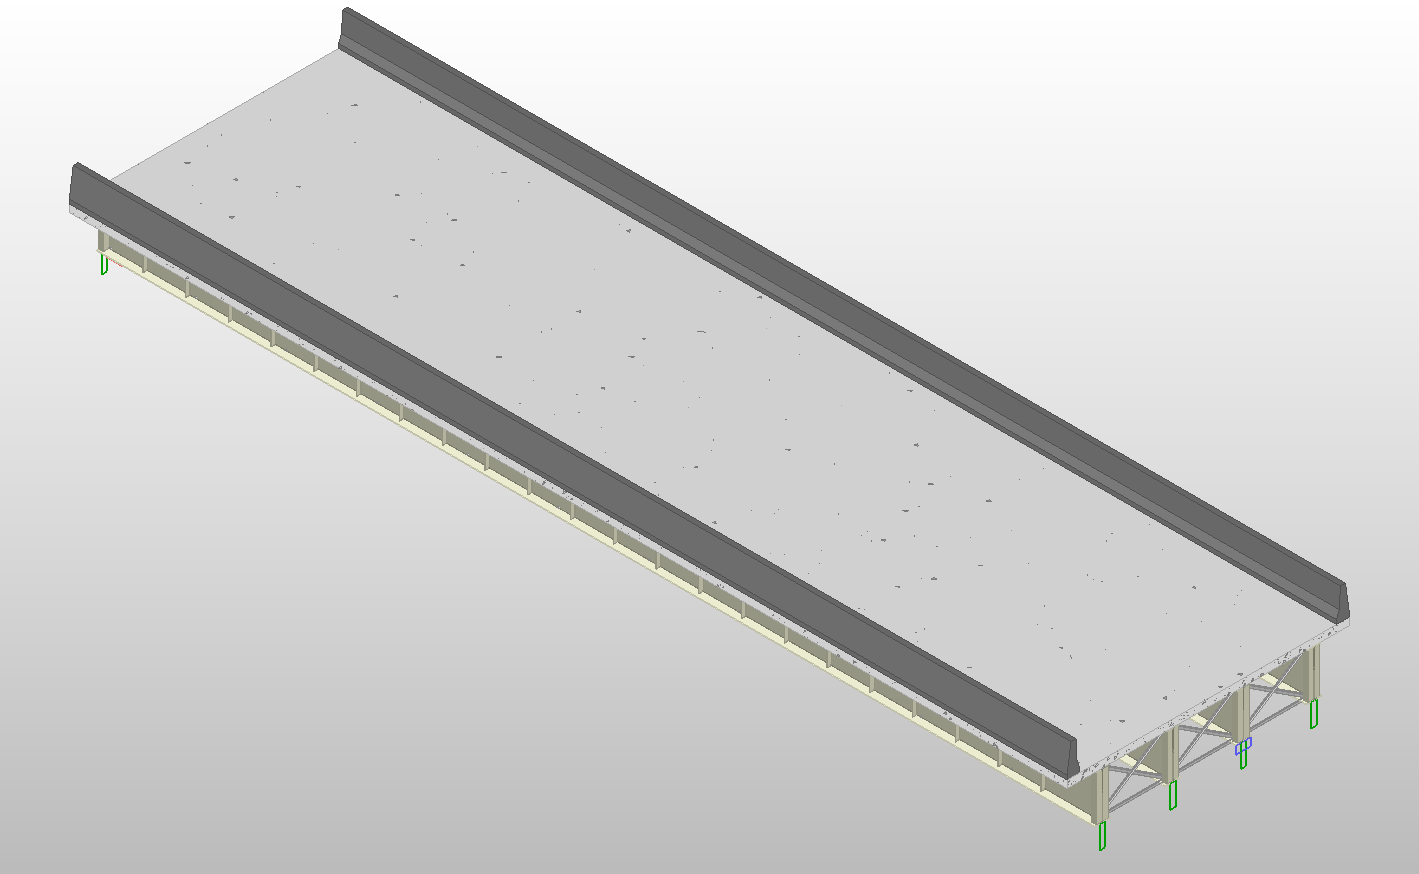
\includegraphics[width=\linewidth]{S3/TC10/cad3d.png}\caption{TC10: girder D 1600 mm, as designed}\end{subfigure}\hfill
\begin{subfigure}[t]{0.48\linewidth}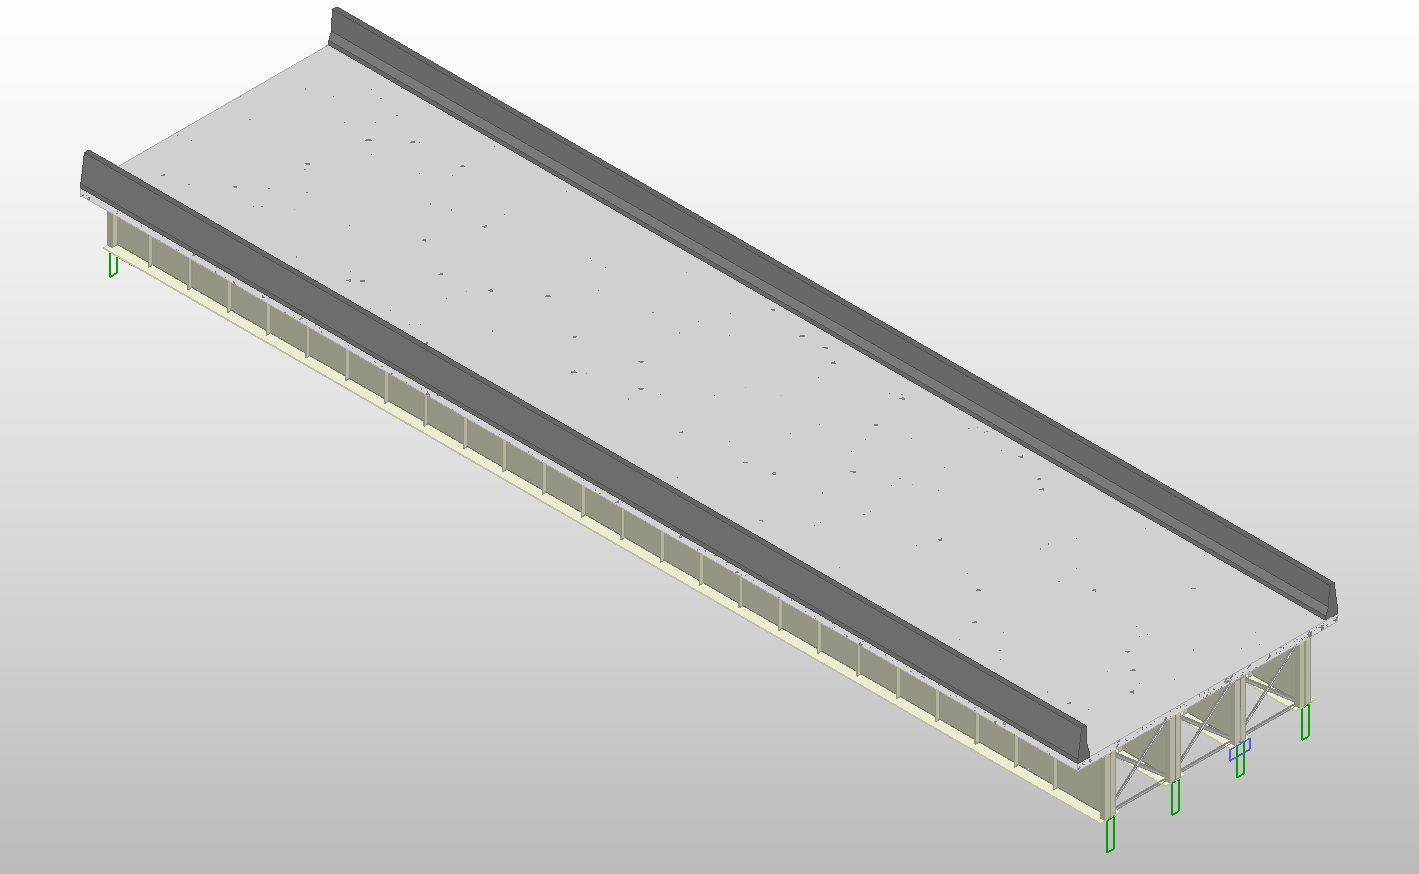
\includegraphics[width=\linewidth]{S3/TC11/cad3d.png}\caption{TC11 after a span change only: drawn D 2120 mm, checked D 1600 mm (\issue{150})}\end{subfigure}
\caption{State carried between runs.}\label{fig:state}
\end{figure}

\section{Graphical outputs}\label{sec:graphics}
Table~\ref{tab:cad} compares the parameters passed to the 3D viewer with the design, and Figures~\ref{fig:views}
and~\ref{fig:dialogs} show the other graphical outputs.
\begin{itemize}
\item The girder drawn matches the girder designed in 14 of 15 runs; TC11 is the exception (\issue{150}).
\item Cross-bracing spacing is always drawn at 3.0 m (\issue{93}), while the inputs hold span/2 and the plan view labels 3.50 m.
  The bracing sections are hard-coded: angle 100$\times$50$\times$8 against a designed 40$\times$40$\times$3 and an input IS
  100$\times$100$\times$10 double angle (comment on \issue{93}).
\item The 3D legend width omits the median: 26.45 m against a 27.85 m layout in TC03 and TC17 (\issue{124}).
\item Shear force and bending moment plots, the cross-section and the plan view rendered for every run and changed with the
  inputs. The design summary dialogs open with the run's values.
\end{itemize}

\begin{table}[htbp]\centering
\caption{3D CAD DTO against the design. Girder: $D \times b_{f,top} \times t_{f,top} \times b_{f,bot} \times t_{f,bot}
\times t_w$. CB = cross bracing, L = angle. The width columns compare the 3D legend with the layout $(n-1)s + 2\,\text{overhang}$.}\label{tab:cad}
{\scriptsize\setlength{\tabcolsep}{3pt}\begin{tabular}{@{}llllll@{}}
\toprule
\textbf{Case} & \textbf{\makecell[l]{Girder designed\\(mm)}} & \textbf{\makecell[l]{Girder drawn\\(mm)}} & \textbf{\makecell[l]{CB spacing (m)\\input / drawn}} & \textbf{\makecell[l]{CB section\\designed / drawn}} & \textbf{\makecell[l]{Width (m)\\legend / layout}} \\
\midrule
TC01 & 1670\texttimes 510\texttimes 22\texttimes 510\texttimes 22\texttimes 10 & same & 15 / 3.0 & 40\texttimes 40\texttimes 3 / L100\texttimes 50\texttimes 8 & 8.4 / 8.4 \\
TC02 & 2230\texttimes 670\texttimes 28\texttimes 670\texttimes 28\texttimes 12 & same & 20 / 3.0 & 40\texttimes 40\texttimes 3 / L100\texttimes 50\texttimes 8 & 10.18 / 10.275 \\
TC03 & 2230\texttimes 670\texttimes 28\texttimes 670\texttimes 28\texttimes 12 & same & 20 / 3.0 & 60\texttimes 60\texttimes 4 / L100\texttimes 50\texttimes 8 & 26.45 / 27.85 \\
TC04 & 1120\texttimes 340\texttimes 16\texttimes 340\texttimes 16\texttimes 8 & same & 10 / 3.0 & 40\texttimes 40\texttimes 3 / L100\texttimes 50\texttimes 8 & 8.4 / 8.4 \\
TC05 & 1390\texttimes 420\texttimes 18\texttimes 420\texttimes 18\texttimes 8 & same & 12.5 / 3.0 & 40\texttimes 40\texttimes 3 / L100\texttimes 50\texttimes 8 & 8.4 / 8.4 \\
TC06 & 1390\texttimes 420\texttimes 18\texttimes 420\texttimes 18\texttimes 8 & same & 12.5 / 3.0 & 40\texttimes 40\texttimes 3 / L100\texttimes 50\texttimes 8 & 8.4 / 8.4 \\
TC07 & 1390\texttimes 420\texttimes 18\texttimes 420\texttimes 18\texttimes 8 & same & 12.5 / 3.0 & 40\texttimes 40\texttimes 3 / L100\texttimes 50\texttimes 8 & 8.4 / 8.4 \\
TC08 & 1390\texttimes 420\texttimes 18\texttimes 420\texttimes 18\texttimes 8 & same & 12.5 / 3.0 & 40\texttimes 40\texttimes 3 / L100\texttimes 50\texttimes 8 & 8.4 / 8.4 \\
TC09 & 1800\texttimes 450\texttimes 25\texttimes 550\texttimes 32\texttimes 14 & same & 17.5 / 3.0 & 40\texttimes 40\texttimes 3 / L100\texttimes 50\texttimes 8 & 9.9 / 9.9 \\
TC10 & 1600\texttimes 450\texttimes 25\texttimes 550\texttimes 32\texttimes 14 & same & 17.5 / 3.0 & 40\texttimes 40\texttimes 3 / L100\texttimes 50\texttimes 8 & 9.9 / 9.9 \\
TC11 & 1600\texttimes 450\texttimes 25\texttimes 550\texttimes 32\texttimes 14 & 2120\texttimes 640\texttimes 28\texttimes 750\texttimes 32\texttimes 12 & 19 / 3.0 & 40\texttimes 40\texttimes 3 / L100\texttimes 50\texttimes 8 & 9.9 / 9.9 \\
TC17 & 2230\texttimes 670\texttimes 28\texttimes 670\texttimes 28\texttimes 12 & same & 20 / 3.0 & 50\texttimes 50\texttimes 3 / L100\texttimes 50\texttimes 8 & 26.45 / 27.85 \\
TC18 & 1670\texttimes 510\texttimes 22\texttimes 510\texttimes 22\texttimes 10 & same & 15 / 3.0 & 40\texttimes 40\texttimes 3 / L100\texttimes 50\texttimes 8 & 8.4 / 8.4 \\
TC19 & 2230\texttimes 670\texttimes 28\texttimes 670\texttimes 28\texttimes 12 & same & 20 / 3.0 & None / L100\texttimes 50\texttimes 8 & 26.45 / 27.85 \\
TC20 & 1670\texttimes 510\texttimes 22\texttimes 510\texttimes 22\texttimes 10 & same & 15 / 3.0 & 40\texttimes 40\texttimes 3 / L100\texttimes 50\texttimes 8 & 8.4 / 8.4 \\
\bottomrule
\end{tabular}
}
\end{table}

\begin{figure}[htbp]\centering
\begin{subfigure}[t]{0.49\linewidth}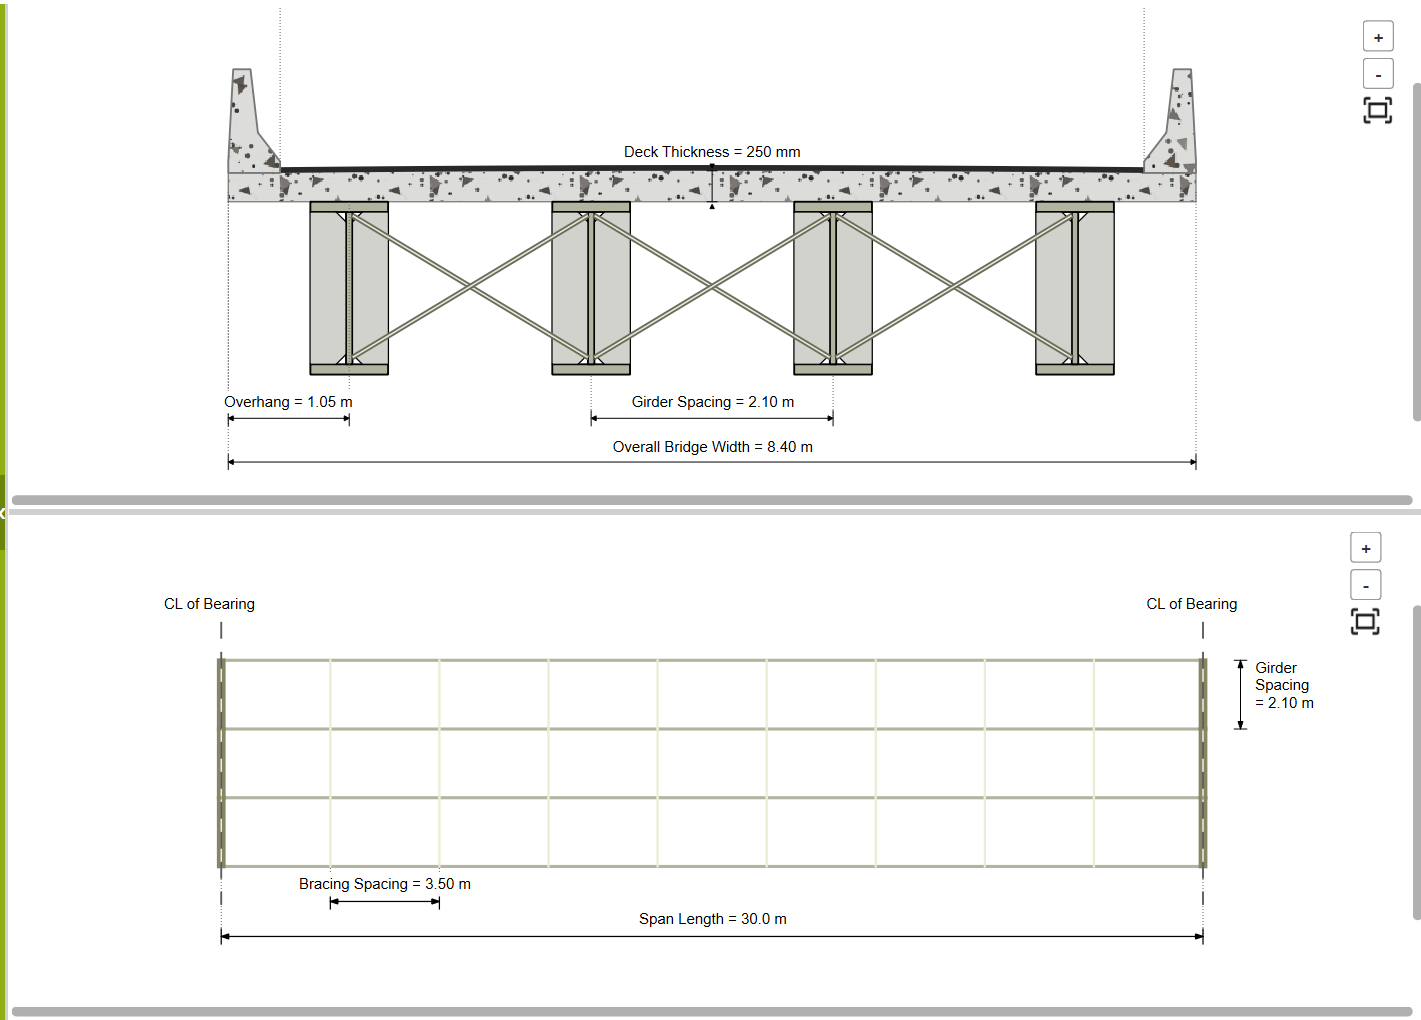
\includegraphics[width=\linewidth]{figures/tc01_xsec_crop.png}\caption{Cross-section and plan (TC01)}\end{subfigure}\hfill
\begin{subfigure}[t]{0.49\linewidth}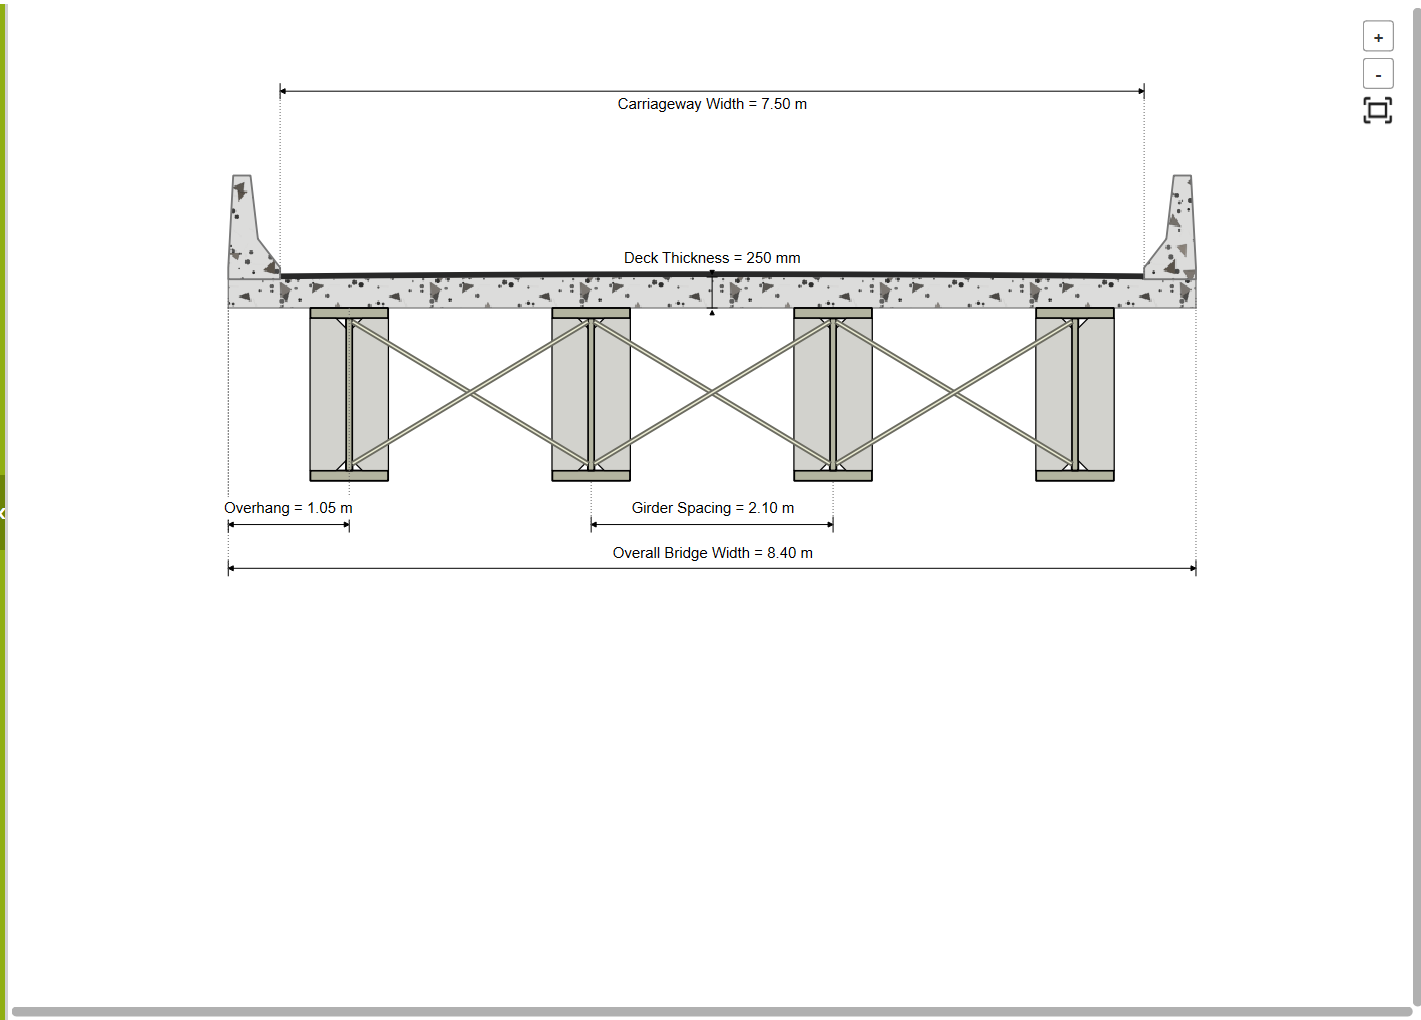
\includegraphics[width=\linewidth]{figures/tc01_top_crop.png}\caption{Typical section with dimensions (TC01)}\end{subfigure}\\[6pt]
\begin{subfigure}[t]{0.49\linewidth}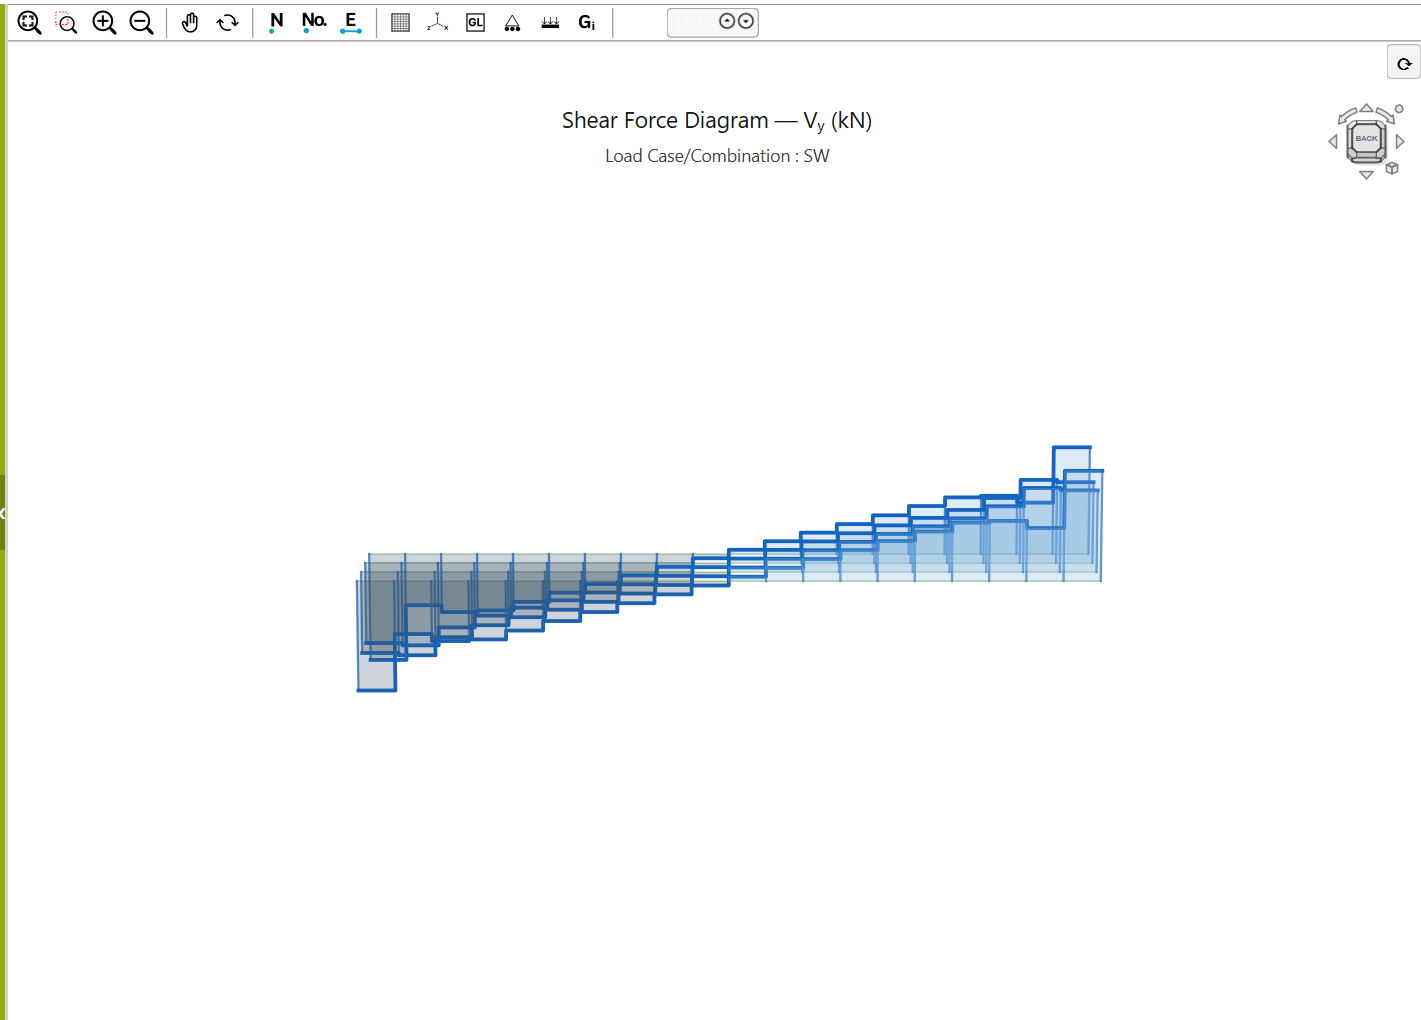
\includegraphics[width=\linewidth]{figures/tc01_sfd_crop.png}\caption{Shear force diagram, load case SW (TC01)}\end{subfigure}\hfill
\begin{subfigure}[t]{0.49\linewidth}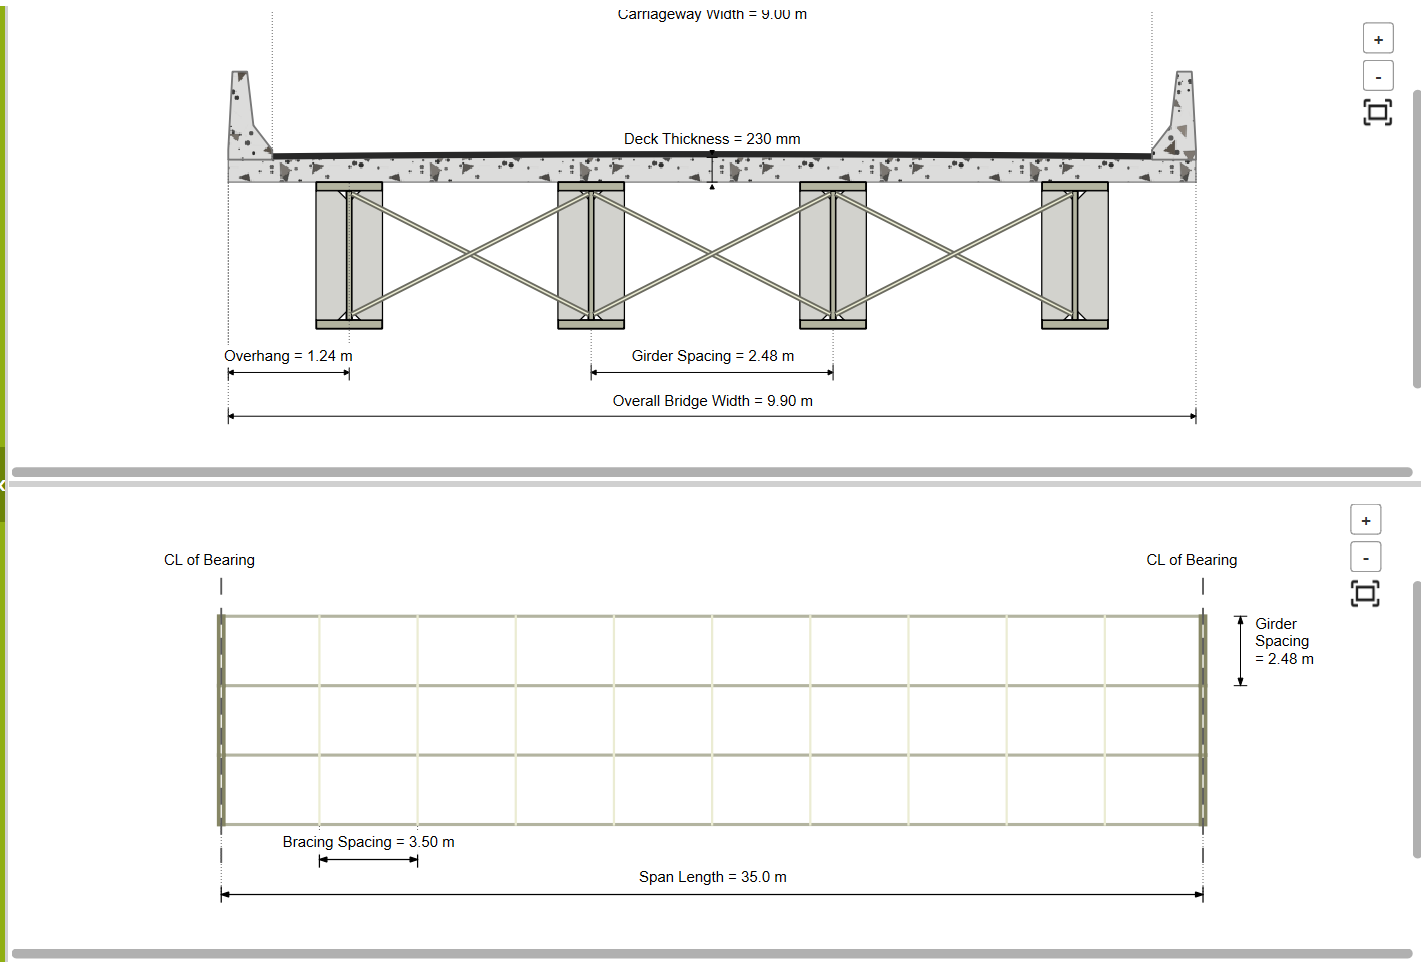
\includegraphics[width=\linewidth]{figures/tc09_xsec_crop.png}\caption{Custom-mode design, deck 230 mm (TC09)}\end{subfigure}
\caption{2D drawings and analysis plots generated by the application.}\label{fig:views}
\end{figure}

\begin{figure}[htbp]\centering
\begin{subfigure}[t]{0.48\linewidth}\centering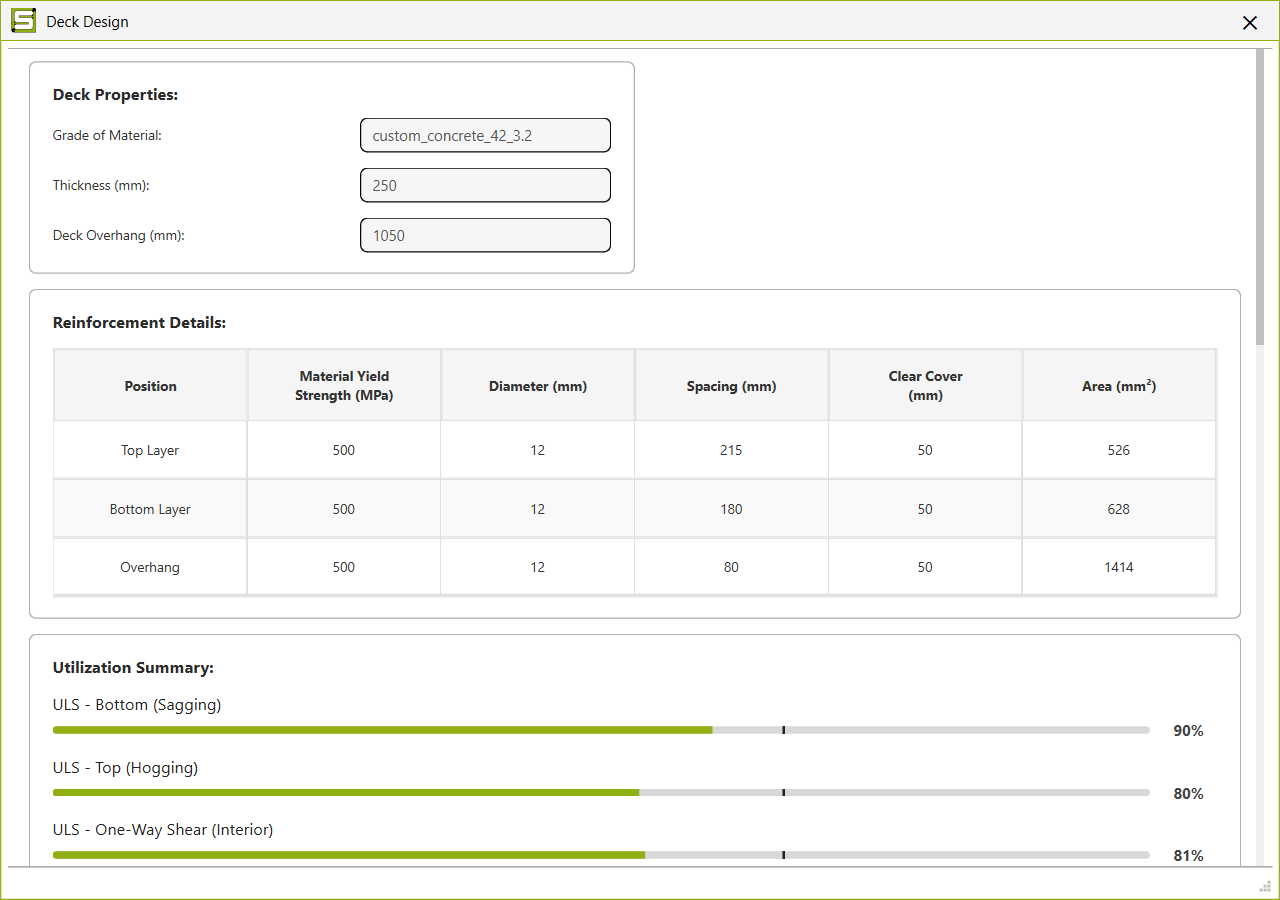
\includegraphics[width=\linewidth]{demo/deck_design_run1.png}\caption{Deck Design summary (demo run 1)}\end{subfigure}\hfill
\begin{subfigure}[t]{0.48\linewidth}\centering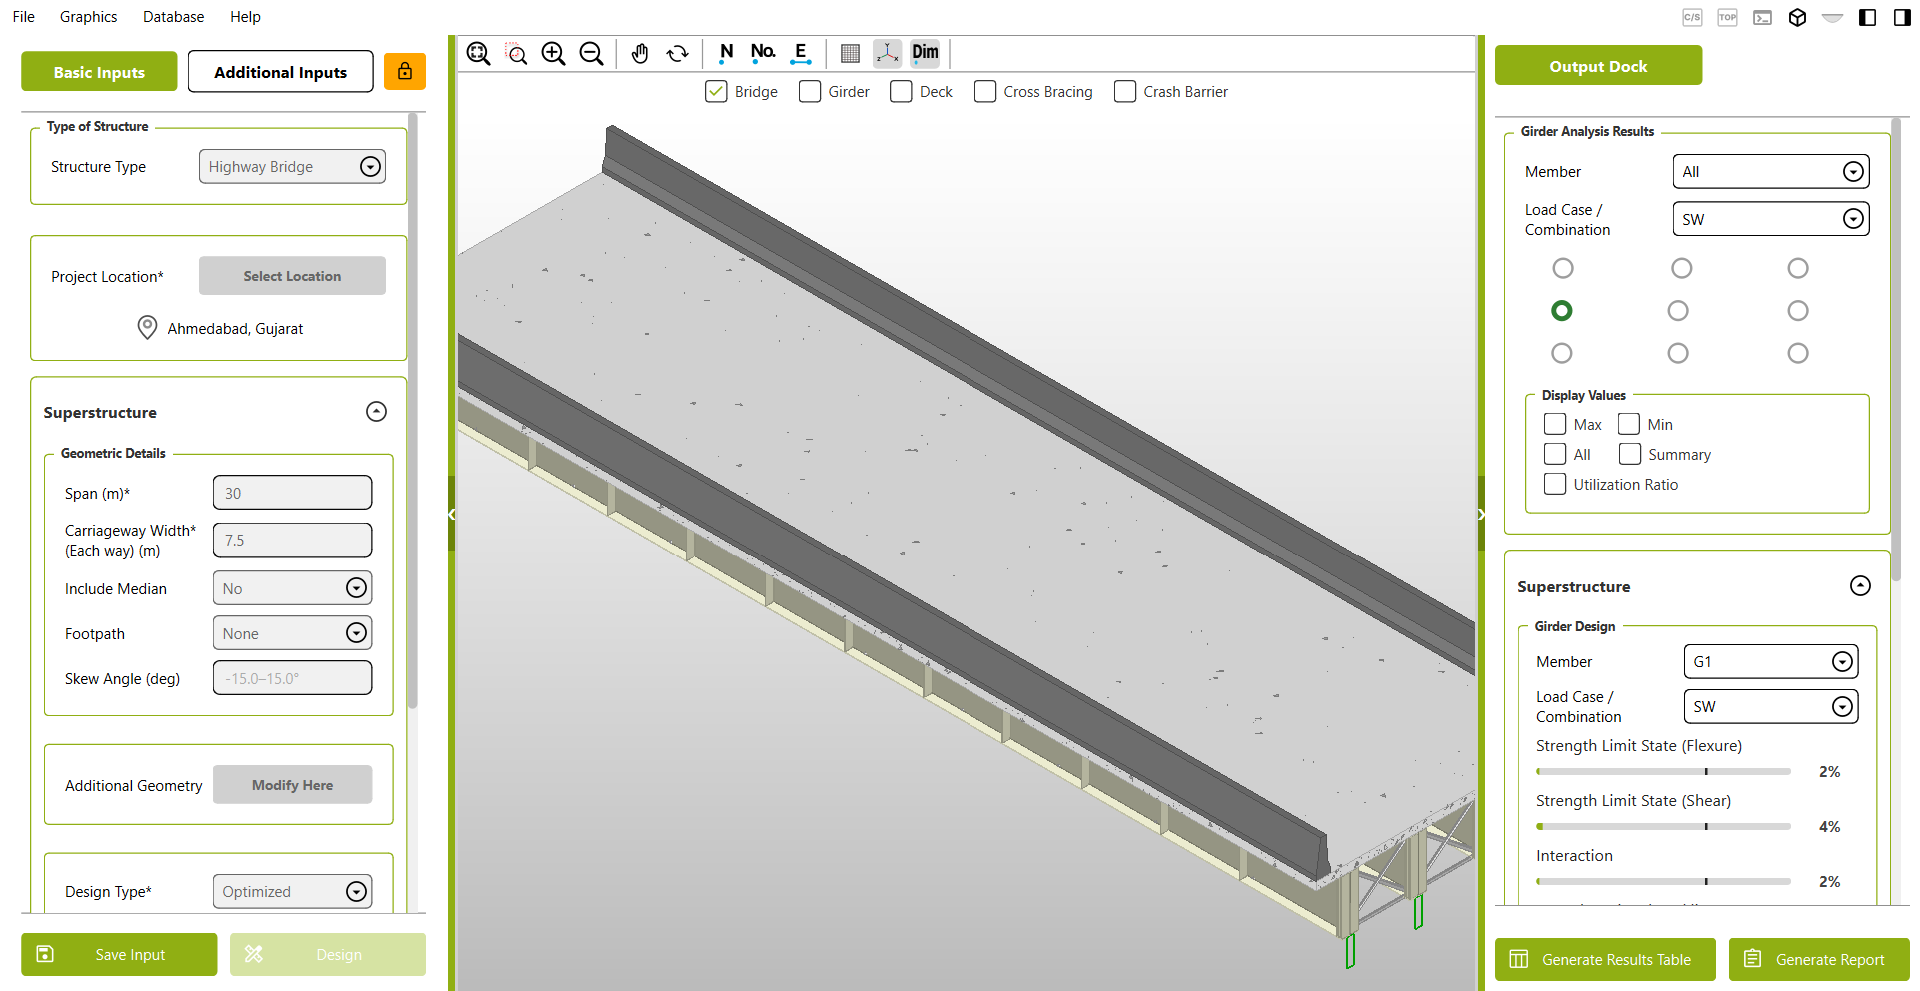
\includegraphics[width=\linewidth]{demo/output_dock_run1.png}\caption{Output Dock after Design (demo run 1)}\end{subfigure}\\[6pt]
\begin{subfigure}[t]{\linewidth}\centering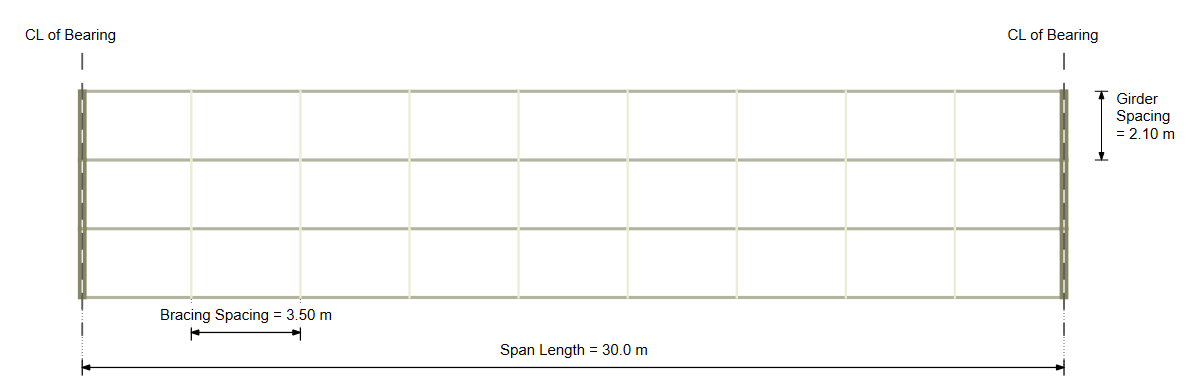
\includegraphics[width=0.66\linewidth]{figures/tc01_plan_view.png}\caption{TC01 plan view labels ``Bracing Spacing = 3.50 m''; the design uses 3.0 m, the inputs 15 m (\issue{93})}\end{subfigure}
\caption{Result dialogs and the 2D plan view.}\label{fig:dialogs}
\end{figure}

% =====================================================================
\section{Issues raised}\label{sec:issues}
Table~\ref{tab:issues} lists the six new issues, the five comments on existing issues and the pull request for \#148. Each
issue on GitHub gives the exact inputs, the captured
dictionaries and probe output as evidence, the root cause with source links pinned to \texttt{d74f56d}, a suggested fix and a
duplicate check. The subsections below summarise each one.

{\small
\begin{longtable}{@{}L{0.07\linewidth}L{0.38\linewidth}L{0.49\linewidth}@{}}
\caption{Issues filed, comments posted and pull request opened on Nidhikhare12/OsdagBridge.}\label{tab:issues}\\
\toprule
\textbf{Issue} & \textbf{Defect} & \textbf{Root cause and proposed fix} \\
\midrule\endfirsthead
\toprule
\textbf{Issue} & \textbf{Defect} & \textbf{Root cause and proposed fix} \\
\midrule\endhead
\issue{147} & Fatigue stress range doubled: report and output dict FAIL 1.58, GUI PASS 0.79 &
\texttt{designer.py} L2970--2994 mixes opposite-signed $M_{z,i}$/$M_{z,j}$. Negate the j-end, take the range per section. \\
\issue{148} & Deck SLS checks with $E_{cm}$ in GPa: $\alpha_e$ 6061, $\sigma_c$ 4$\times$ low, $w_k$ 25\,\% low &
\texttt{plategirderbridge.py} L3186. Pass \texttt{Ecm * 1000} to \texttt{deckdesign}. \\
\issue{149} & Same-Fy/Fu custom steels collide; the girder silently takes the CB's E and density &
\texttt{material\_properties.py} L689 names from Fy/Fu only; \texttt{input\_dock.py} L736 overwrites. Use unique names. \\
\issue{150} & Custom mode: after a span change the CAD, edge lines and deck use the initial-sizing girder &
\texttt{defaults.py} L647--650 re-seeds base keys; \texttt{resolve\_girder\_value} prefers them. Sync base keys from G1.M1. \\
\issue{151} & Report Tables 5.1--5.6 repeat the controlling girder; \texttt{util.*} hides worse girders &
\texttt{chap5.py} L170--260 renders scalar keys per row. Read \texttt{per\_girder}, take the max per category. \\
\issue{152} & AttributeError on every Footpath change &
\texttt{input\_dock.py} L666 calls a method removed in \texttt{cacaada}. Delete the call. \\
\midrule
\issue{20} & Comment: self-weight never uses \texttt{steel\_prop.rho} & \texttt{analyser.py} L416 uses the 78.5 constant. \\
\issue{20} & Comment: correction of identifiers cited in a later comment & No \texttt{steel\_density} key exists;
\texttt{SteelProperties} is frozen; the self-weight ignores \texttt{rho}. \\
\issue{93} & Comment: CB and ED sections hard-coded in CAD & \texttt{plategirderbridge.py} L3368--3369, L3590--3625. \\
\issue{112} & Comment: median/footpath changes and consecutive runs & 7 m spacing accepted; 7 girders kept on 8.4 m. \\
\issue{134} & Comment: GUI reproduction at cw 11 m & Dock and output dict disagree when the live load is dropped. \\
\midrule
\issue{235} & Pull request: fix for \#148 & \texttt{Ecm * 1000.0} at the \texttt{deckdesign} call, with a regression test. \\
\bottomrule
\end{longtable}}

\subsection{\#147 Girder fatigue stress range is doubled}\label{sec:i147}
\textbf{Works / fails.} The Output Dock and the Design Check tab are correct. The output dictionary, the Executive Summary and
report Table 5.12 are wrong in every run that has a fatigue check (14 of 15), by exactly 2.00.\\
\textbf{Evidence (TC01, G3).} Dock 79\,\%; Design Check $\Delta\sigma$ = 72.93 MPa / 92.49 MPa = 0.79 PASS;
\texttt{util.fatigue} = 157.70; report 145.86 MPa, UR 1.577 FAIL. Probe output:
\code{snippets/fatigue_excerpt.txt}
\textbf{Root cause.} \src{designer.py} L2970--2994 (\texttt{\_extract\_demands\_from\_analysis\_results}, step 4) concatenates the
$M_{z,i}$ and $M_{z,j}$ element end forces and takes max $-$ min. The two ends use opposite signs for the same internal moment,
so max $-$ min $= 2|M|$. The per-load-case path (L3082--3083) uses $\max(|M_{z,i}|, |M_{z,j}|)$ and feeds the dock.\\
\textbf{Suggested fix.}
\code{snippets/fix_147.txt}

\subsection{\#148 Deck slab SLS checks use $E_{cm}$ in GPa as if it were MPa}
\textbf{Works / fails.} The girder design is correct (\src{designer.py} L336--337 converts with \texttt{* 1000}). The deck slab
path is wrong for database grades and custom concrete alike (TC01, TC05, TC09).\\
\textbf{Evidence (TC01, M40, Fe 500).}
\begin{center}\small
\begin{tabular}{@{}lrr@{}}
\toprule
\texttt{deck\_design\_results} & \textbf{As designed ($E_{cm}$ = 33 ``MPa'')} & \textbf{$E_{cm}$ = 33\,000 MPa} \\
\midrule
Modular ratio $\alpha_e$ & 6060.6 & 6.06 \\
Neutral axis $x/d$ (bottom mat) & 0.976 & 0.182 \\
Concrete stress $\sigma_c$ bottom, UR & 2.49 MPa, 0.13 & 9.84 MPa, 0.51 \\
Steel stress $\sigma_s$ bottom, UR & 365.3 MPa, 0.913 & 276.9 MPa, 0.692 \\
Crack width bottom / top & 0.198 / 0.213 mm & 0.263 / 0.281 mm \\
Bottom reinforcement & $\phi$12 @ 175 & $\phi$12 @ 185 \\
\bottomrule
\end{tabular}
\end{center}
\textbf{Root cause.} \src{plategirderbridge.py} L3185--3196 passes \texttt{concrete\_prop.Ecm}, which is in GPa (\src{dto.py}
L146). \src{deckdesign.py} L429--430 documents MPa and \texttt{\_cracked\_section()} L211 computes
\texttt{alpha\_e = Es\_MPa / Ecm\_MPa}.\\
\textbf{Suggested fix.}
\begin{Verbatim}[frame=single,framesep=5pt,fontsize=\footnotesize,samepage=true]
# plategirderbridge.py, design_deck_slab()
Ecm = self.material_props.concrete_prop.Ecm * 1000.0   # GPa -> MPa (deckdesign expects MPa)
\end{Verbatim}
\textbf{Fix.} Pull request \issue{235} makes this change and adds \texttt{tests/unit/test\_deck\_ecm\_units.py}, which fails on
\texttt{dev} and passes with the fix. Full designs of TC01, TC05 and TC09 on the fix branch reproduce the right-hand column
above. Every deck check still passes (highest UR 0.99), and the girder utilisations do not change.

\subsection{\#149 Two custom steels with the same Fy/Fu collide}
\textbf{Works / fails.} Works while every custom steel has a distinct Fy/Fu pair. Fails when two coincide: TC06 girder custom
(Fy 410, Fu 540, E 210, $\rho$ 80); TC08 cross bracing custom (Fy 410, Fu 540, E 200, $\rho$ 77). Both are named
\texttt{custom\_steel\_410\_540}; at the next Design the girder silently takes E = 200 GPa and $\rho$ = 77.\\
\textbf{Root cause.} \src{material\_properties.py} L672--689 builds the name from Fy and Fu only; \src{input\_dock.py} L736
stores \texttt{\_material\_custom\_fields[name]}, replacing the first entry; \texttt{\_prime\_material\_inputs()} (L324--345, run
on every Design) re-exports it to every member showing that name.\\
\textbf{Suggested fix.} Give a material with different properties a distinct name:
\begin{Verbatim}[frame=single,framesep=5pt,fontsize=\footnotesize,samepage=true]
# input_dock.py, _on_material_changed(), after the dialog is accepted
fields = dict(fd.get("fields") or {})
stored = self._material_custom_fields.get(mat)
if stored is not None and stored != fields:      # same Fy/Fu, different E / density
    n = 2
    while f"{mat}_{n}" in self._material_custom_fields:
        n += 1
    mat = f"{mat}_{n}"                           # e.g. custom_steel_410_540_2
self._material_custom_fields[mat] = fields
\end{Verbatim}

\subsection{\#150 Custom mode: CAD and edge lines use the initial-sizing girder after a span change}
\textbf{Works / fails.} Works in the first Custom run (TC09) and when only Additional Inputs change (TC10). Fails from the
first Design after a homepage field changes (TC11, span 35 $\rightarrow$ 38): the per-girder keys keep the user's
1600$\times$450$\times$25 / 550$\times$32, $t_w$ 14 section, but the base keys are re-seeded with the initial-sizing
2120$\times$640$\times$28 / 750$\times$32, $t_w$ 12 section, which the CAD, the grillage edge lines, design lines 5--6 and the
deck design then use (Figure~\ref{fig:state}).
\code{snippets/base_keys_excerpt.txt}
\textbf{Root cause.} \src{defaults.py} L644--650 overwrites all base keys unconditionally; \texttt{resolve\_girder\_value}
(\src{plategirderbridge.py} L289--314) tries the base key before \texttt{.G1.M1} when no girder index is given.\\
\textbf{Suggested fix.}
\begin{Verbatim}[frame=single,framesep=5pt,fontsize=\footnotesize,samepage=true]
# defaults.py, _on_no_of_girders_changed(): keep base keys in step with G1 in Custom mode
for base_key, value in MP_GIRDER_PROPS:
    g1 = working_input_dict.get(f"{base_key}.G1.M1")
    keep_seed = design_mode == "Optimized" or g1 in (None, "", "All")
    working_input_dict[base_key] = value if keep_seed else g1

# plategirderbridge.py, resolve_girder_value(): prefer the per-girder key
candidates = ([f"{base_key}.G{i + 1}.M1"] if i is not None else []) \
             + [f"{base_key}.G1.M1", base_key]
\end{Verbatim}

\subsection{\#151 Report per-girder tables repeat the controlling girder}
\textbf{Works / fails.} The Output Dock and Design Check show each girder correctly. Report Tables 5.1--5.6 print the
controlling girder (highest overall DCR) in every girder block, and \texttt{util.*} reports only that girder per category.\\
\textbf{Evidence.} TC01: Vu printed 288.29 kN in every row against 379.98 kN for the exterior lines in \texttt{per\_girder};
\texttt{util.shear} 40.03\,\% against a worst dock bar of 52.76\,\% (G2). The report understates the worst shear by 32\,\%. TC09:
383.37 kN printed against 517.22 kN.\\
\textbf{Root cause.} \src{chap5.py} L170--260 loops over girders but renders scalar keys (\texttt{KEY\_SD\_SHEAR\_VU},
\texttt{KEY\_UTIL\_SHEAR}, \ldots) written once from the controlling girder by \texttt{store\_design\_results()}
(\src{plategirderbridge.py} L4102--4109).\\
\textbf{Suggested fix.} Read each row from \texttt{design\_results["per\_girder"]} and write \texttt{util.<category>} as the
maximum over girders:
\begin{Verbatim}[frame=single,framesep=5pt,fontsize=\footnotesize,samepage=true]
# plategirderbridge.py, store_design_results()
per = dr["per_girder"].values()
worst = lambda cat: max((g["category_urs"].get(cat, {}).get("max_dcr", 0.0) for g in per),
                        default=0.0)
out[KEY_UTIL_SHEAR] = worst(2) * 100          # likewise for categories 1 and 3-8
\end{Verbatim}

\subsection{\#152 Changing Footpath raises \texttt{AttributeError}}
\textbf{Works / fails.} Designs still complete because Qt swallows the exception, but every Footpath change (9 of 9 across S1,
S5, S6 and the demo) prints a traceback and the intended forwarding never happens.
\begin{Verbatim}[frame=single,framesep=5pt,fontsize=\footnotesize,samepage=true]
File ".../desktop/ui/docks/input_dock.py", line 666, in _on_footpath_changed
    self.parent.notify_additional_inputs_footpath(value)
AttributeError: 'CustomWindow' object has no attribute 'notify_additional_inputs_footpath'
\end{Verbatim}
\textbf{Root cause.} The method was removed from \src{template\_page.py} in commit \texttt{cacaada}; the Additional Inputs dialog
now refreshes the footpath sub-tabs itself when opened.\\
\textbf{Suggested fix.} Delete the call at \src{input\_dock.py} L666.

\subsection{Comments on existing issues}
\begin{itemize}
\item \issue{20}: the self-weight load never reads \texttt{steel\_prop.rho}; \src{analyser.py} L416 uses the constant 78.5, and the
  report states 76.4 kN/m\textsuperscript{3}. Custom densities 80 and 30 had no effect.
\item \issue{93}: the CAD hard-codes the cross-bracing and end-diaphragm sections (\src{plategirderbridge.py} L3368--3369,
  L3590--3625) as well as the spacing.
\item \issue{112}: girder count after median and footpath changes and across consecutive runs (TC03, TC17--TC20).
\item \issue{134}: a GUI reproduction at carriageway 11 m in which the live load is dropped, all demands are zero and the dock and
  output dictionary disagree (TC19).
\item \issue{20} (22 November): a correction to a later comment. That comment cited \texttt{steel\_density},
  \texttt{KEY\_STEEL\_DENSITY} and \texttt{steel\_prop.density}, which do not exist at \texttt{d74f56d}, and proposed
  overwriting a field of the frozen \texttt{SteelProperties}, which raises \texttt{FrozenInstanceError}.
\end{itemize}

\subsection{Duplicate check}
Before filing I searched all 83 open and closed issues (up to \#146) and their comments on 17 and 18 November 2026. Defects that
were already reported (\issue{20}, \issue{41}, \issue{43}, \issue{45}, \issue{66}, \issue{71}, \issue{89}, \issue{112},
\issue{113}, \issue{124}, \issue{134}) received comments only where I had new information. On 22 November I re-checked the
issues opened since, up to \#230. None duplicates mine. Two later ones are related but distinct: \issue{171} (Excel export
labels $E_{cm}$ in GPa as MPa; my \#148 is the deck design calculation itself) and \issue{177} (the shear fatigue limit; my
\#147 is the doubled stress range).

\subsection{Activity since filing (to 22 November 2026)}
\begin{itemize}
\item \issue{148} was reproduced independently on macOS on 20 November, with the same modular ratio and neutral axis. The
  reporter filed the Results Table export part of the same unit error as \issue{171}. I opened \issue{235} with the fix.
\item \issue{20}: another tester's GUI run (22 November) shows \texttt{rho} = 78500 and an unchanged self-weight for a
  78 kN/m\textsuperscript{3} custom steel, which confirms that the density must also reach the self-weight load.
\item \issue{112}: open pull request \issue{220} re-seeds the girder count whenever the overall deck width changes. Its
  tests include median and footpath changes, the cases in my comment.
\item \issue{151} is cited as related by \issue{216} (cross-bracing report tables) and \issue{223} (saved \texttt{.osi}
  section properties).
\item The maintainer has not yet replied to, labelled or assigned \issue{147}--\issue{152}.
\end{itemize}

\needspace{14\baselineskip}
\section{Deliverables}
\begin{table}[htbp]
\small
\begin{tabularx}{\linewidth}{@{}lY@{}}
\toprule
\textbf{Item} & \textbf{Location} \\
\midrule
Test scripts, logs, evidence & \href{https://github.com/Aditya060806/OsdagBridge/tree/screening-testing/testing}{\nolinkurl{Aditya060806/OsdagBridge}}, branch \texttt{screening-testing}, folder \texttt{testing/} \\
Test-case \texttt{.osi} files & \ev{osi} (20 files, all pass \texttt{validate\_osi\_inputs}) \\
Per-case evidence & \ev{results} (dictionaries, dock values, CAD parameters, screenshots, logs) \\
Root-cause probes & \ev{probes} with outputs in \texttt{probes/output/} \\
Issue texts & \ev{issues} and \texttt{issues/published.json} (links) \\
Fix for \#148 & Pull request \issue{235}, branch \texttt{fix/148-deck-ecm-mpa} on the fork \\
This report & \ev{report/report.pdf} (LaTeX source \texttt{report.tex}) \\
Screencast & \ev{results/demo/osdagbridge_testing_demo.mp4}: custom material run, consecutive runs, 3D CAD and plots \\
\bottomrule
\end{tabularx}
\end{table}

\section{Limitations}
\begin{itemize}
\item Inputs were entered by the test driver through the widgets, not by hand. The same code paths run (signals, validators,
  dialogs), but timing-dependent UI glitches would not be seen. The screencast shows the driver at work.
\item Not covered: IFC export, Excel results export, the web and CLI front ends, OSI load and save beyond writing the 20 case files,
  and engineering verification of the IRC 6/22 formulas beyond the defects listed.
\end{itemize}

\appendix
\section{Reproducing the results}
\begin{Verbatim}[frame=single,framesep=6pt,fontsize=\footnotesize]
git clone -b screening-testing https://github.com/Aditya060806/OsdagBridge.git
cd OsdagBridge
conda env create -f environment.yml
conda activate osdagbridge-env
cd testing
python campaign.py S1 S2 S3 S4 S5 S6     # GUI sessions -> results/
python verify.py                         # cross-checks -> report/generated/
python probes/probe_fatigue_range.py results/S1/TC01/input_dict.json
python probes/probe_deck_ecm_units.py results/S1/TC01/input_dict.json
python probes/probe_custom_base_keys.py results/S3/TC11/input_dict.json
python export_osi.py                     # all cases as .osi -> osi/
python demo_video.py                     # screencast -> results/demo/
\end{Verbatim}
\end{document}
